\documentclass[11pt,oneside]{book}

%%%%%%%%%%%%%%%%%%%%%%%%%%%%%%%%%%%%%%%%%%%%%%%%%%%%%%%%%%%%%%%%%%%%%%%%%%%%%%%%%%%%%%%%%%%%%%%%%%%
%                                                                                                 %
% The mathematical style of these documents follows                                               %
%                                                                                                 %
% A. Thompson and B.N. Taylor. The NIST Guide for the Use of the International System of Units.   %
%    NIST Special Publication 881, 2008.                                                          %
%                                                                                                 %
% http://www.nist.gov/pml/pubs/sp811/index.cfm                                                    %
%                                                                                                 %
%%%%%%%%%%%%%%%%%%%%%%%%%%%%%%%%%%%%%%%%%%%%%%%%%%%%%%%%%%%%%%%%%%%%%%%%%%%%%%%%%%%%%%%%%%%%%%%%%%%

% $Date: 2013-11-26 10:43:59 -0500 (Tue, 26 Nov 2013) $
% $Revision: 17538 $
% $Author: gforney $

%%%%%%%%%%%%%%%%%%%%%%%%%%%%%%%%%%%%%%%%%%%%%%%%%%%%%%%%%%%%%%%%%%%%%%%%%%%%%%%%%%%%%%%%%%%%%%%%%%%
%                                                                                                 %
% The mathematical style of these documents follows                                               %
%                                                                                                 %
% A. Thompson and B.N. Taylor. The NIST Guide for the Use of the International System of Units.   %
%    NIST Special Publication 881, 2008.                                                          %
%                                                                                                 %
% http://www.nist.gov/pml/pubs/sp811/index.cfm                                                    %
%                                                                                                 %
%%%%%%%%%%%%%%%%%%%%%%%%%%%%%%%%%%%%%%%%%%%%%%%%%%%%%%%%%%%%%%%%%%%%%%%%%%%%%%%%%%%%%%%%%%%%%%%%%%%

% Packages which force the use of better TeX coding
% Mostly from http://tex.stackexchange.com/q/19264
%%\RequirePackage[l2tabu, orthodox]{nag}
%%\usepackage{fixltx2e}
%\usepackage{isomath} % Disabled for the moment because it changes the syntax for bold and roman Greek math symbols
%%\usepackage[all,warning]{onlyamsmath}
%\usepackage{strict} % Commented out for now because it is uncommon. A copy of style.sty is in Manuals/LaTeX_Style_Files/.

\usepackage{times,mathptmx}
\usepackage[pdftex]{graphicx}
\usepackage{tabularx,ragged2e,booktabs,caption}
\usepackage{multirow}
\usepackage{pdfsync}
\usepackage{tikz}
\usepackage{pgfplots}
%\pgfplotsset{compat=1.7}
\usepackage{tocloft}
\usepackage{color}
\usepackage{amsmath}
\definecolor{linknavy}{rgb}{0,0,0.50196}
\definecolor{linkred}{rgb}{1,0,0}
\definecolor{linkblue}{rgb}{0,0,1}
\usepackage{float}
\usepackage{caption}
\usepackage{graphpap}
\usepackage{rotating}
\usepackage{graphicx}
\usepackage{geometry}
\usepackage{relsize}
\usepackage{longtable}
\usepackage{lscape}
\usepackage{amssymb}
\usepackage{makeidx} % Create index at end of document
\usepackage[nottoc,notlof,notlot]{tocbibind} % Put the bibliography and index in the ToC
\usepackage{lastpage} % Automatic last page number reference.
\usepackage[T1]{fontenc}
\usepackage{enumerate}
\usepackage{upquote}
\usepackage{moreverb}
\usepackage{xfrac}
\usepackage{cite}

\newcommand{\nopart}{\expandafter\def\csname Parent-1\endcsname{}} % To fix table of contents in pdf.
\newcommand{\ct}{\tt\small} % eventually will be deprecated due to http://www.tex.ac.uk/cgi-bin/texfaq2html?label=2letterfontcmd
\newcommand{\textct}[1]{\texttt{\small #1}}

\usepackage{tocstyle} % Fix table of contents sections from overlapping section titles
\usetocstyle{standard}
\usepackage{siunitx}
\sisetup{
    detect-all = true,
    input-decimal-markers = {.},
    input-ignore = {,},
    inter-unit-product = \ensuremath{{}\cdot{}},
    multi-part-units = repeat,
    number-unit-product = \text{~},
    per-mode = fraction,
    separate-uncertainty = true,
}

\usepackage{listings}
\usepackage{textcomp}
\definecolor{lbcolor}{rgb}{0.96,0.96,0.96}
\lstset{
    %backgroundcolor=\color{lbcolor},
    tabsize=4,
    rulecolor=,
    language=Fortran,
        basicstyle=\footnotesize\ttfamily,
        upquote=true,
        aboveskip={\baselineskip},
        belowskip={\baselineskip},
        columns=fixed,
        extendedchars=true,
        breaklines=true,
        breakatwhitespace=true,
        frame=none,
        showtabs=false,
        showspaces=false,
        showstringspaces=false,
        identifierstyle=\ttfamily,
        keywordstyle=\color[rgb]{0,0,0},
        commentstyle=\color[rgb]{0,0,0},
        stringstyle=\color[rgb]{0,0,0},
}

\usepackage[pdftex,
        colorlinks=true,
        urlcolor=linkblue,     % \href{...}{...} external (URL)
        citecolor=linkred,     % citation number colors
        linkcolor=linknavy,    % \ref{...} and \pageref{...}
        pdfproducer={pdflatex},
        pdfpagemode=UseNone,
        bookmarksopen=true,
        plainpages=false,
        verbose]{hyperref}

% The Following commented code makes the ``Draft'' watermark on each page.
%\usepackage{eso-pic}
%\usepackage{type1cm}
%\makeatletter
%   \AddToShipoutPicture{
%     \setlength{\@tempdimb}{.5\paperwidth}
%     \setlength{\@tempdimc}{.5\paperheight}
%     \setlength{\unitlength}{1pt}
%     \put(\strip@pt\@tempdimb,\strip@pt\@tempdimc){
%     \makebox(0,0){\rotatebox{45}{\textcolor[gray]{0.75}{\fontsize{8cm}\selectfont{RC6}}}}}
% }
%\makeatother

\setlength{\textwidth}{6.5in}
\setlength{\textheight}{9.0in}
\setlength{\topmargin}{0.in}
\setlength{\headheight}{0.pt}
\setlength{\headsep}{0.in}
\setlength{\parindent}{0.25in}
\setlength{\oddsidemargin}{0.0in}
\setlength{\evensidemargin}{0.0in}
\setlength{\leftmargini}{\parindent} % Controls the indenting of the "bullets" in a list
\setlength{\cftsecnumwidth}{0.45in}
\setlength{\cftsubsecnumwidth}{0.5in}
\setlength{\cftfignumwidth}{0.45in}
\setlength{\cfttabnumwidth}{0.45in}

\newcommand{\titlesigs}
{
\small
\flushright{U.S. Department of Commerce \\
{\em Penny Pritzker, Secretary} \\
\hspace{1in} \\
National Institute of Standards and Technology \\
{\em Willie May, Under Secretary of Commerce for Standards and Technology and Acting Director} }
}

% commands to use for "official" cover and title pages
% see smokeview verification guide to see how they are used

\newcommand{\headerA}[1]{
\flushright{
\fontsize{20}{24}\selectfont
\bf{NIST Special Publication #1}}
}

\newcommand{\headerB}[1]{
\flushright{
\fontsize{28}{33.6}\selectfont
\bf{#1}
}
}

\newcommand{\headerC}[1]{
\vspace{.5in}
\flushright{\fontsize{14}{16.8}\selectfont
#1}
}

\frenchspacing

\newcommand{\dod}[2]{\frac{\partial #1}{\partial #2}}
\newcommand{\DoD}[2]{\frac{\mathrm{D} #1}{\mathrm{D} #2}}
\newcommand{\dsods}[2]{\frac{\partial^2 #1}{\partial #2^2}}
\renewcommand{\d}{\,\mathrm{d}}
\newcommand{\dx}{\delta x}
\newcommand{\dy}{\delta y}
\newcommand{\dz}{\delta z}
\newcommand{\degF}{$^\circ$F}
\newcommand{\degC}{$^\circ$C}
\newcommand{\x}{x}
\newcommand{\y}{y}
\newcommand{\z}{z}
\newcommand{\dt}{\delta t}
\newcommand{\dn}{\delta n}
\newcommand{\cH}{H}
\newcommand{\hu}{u}
\newcommand{\hv}{v}
\newcommand{\hw}{w}
\newcommand{\la}{\lambda}
\newcommand{\bO}{{\Omega}}
\newcommand{\bo}{{\mathbf{\omega}}}
\newcommand{\btau}{\mathbf{\tau}}
\newcommand{\bdelta}{{\mathbf{\delta}}}
\newcommand{\sumyw}{\sum (Y_\alpha/W_\alpha)}
\newcommand{\oW}{\overline{W}}
\newcommand{\om}{\ensuremath{\omega}}
\newcommand{\omx}{\omega_x}
\newcommand{\omy}{\omega_y}
\newcommand{\omz}{\omega_z}
\newcommand{\erf}{\hbox{erf}}
\newcommand{\erfc}{\hbox{erfc}}
\newcommand{\bF}{{\mathbf{F}}}
\newcommand{\bG}{{\mathbf{G}}}
\newcommand{\bof}{{\mathbf{f}}}
\newcommand{\bq}{{\mathbf{q}}}
\newcommand{\br}{{\mathbf{r}}}
\newcommand{\bu}{{\mathbf{u}}}
\newcommand{\bx}{{\mathbf{x}}}
\newcommand{\bk}{{\mathbf{k}}}
\newcommand{\bv}{{\mathbf{v}}}
\newcommand{\bg}{{\mathbf{g}}}
\newcommand{\bn}{{\mathbf{n}}}
\newcommand{\bS}{{\mathbf{S}}}
\newcommand{\bW}{\overline{W}}
\newcommand{\dS}{d{\mathbf{S}}}
\newcommand{\bs}{{\mathbf{s}}}
\newcommand{\bI}{{\mathbf{I}}}
\newcommand{\hp}{H}
\newcommand{\trho}{\tilde{\rho}}
\newcommand{\dph}{{\delta\phi}}
\newcommand{\dth}{{\delta\theta}}
\newcommand{\tp}{\tilde{p}}
\newcommand{\bp}{\overline{p}}
\newcommand{\dQ}{\dot{Q}}
\newcommand{\dq}{\dot{q}}
\newcommand{\dbq}{\dot{\mathbf{q}}}
\newcommand{\dm}{\dot{m}}
\newcommand{\ha}{\frac{1}{2}}
\newcommand{\ft}{\frac{4}{3}}
\newcommand{\ot}{\frac{1}{3}}
\newcommand{\fofi}{\frac{4}{5}}
\newcommand{\of}{\frac{1}{4}}
\newcommand{\twth}{\frac{2}{3}}
\newcommand{\R}{R}
\newcommand{\be}{\begin{equation}}
\newcommand{\ee}{\end{equation}}
\newcommand{\RE}{\hbox{Re}}
\newcommand{\LE}{\hbox{Le}}
\newcommand{\PR}{\hbox{Pr}}
\newcommand{\PE}{\hbox{Pe}}
\newcommand{\NU}{\hbox{Nu}}
\newcommand{\SC}{\hbox{Sc}}
\newcommand{\SH}{\hbox{Sh}}
\newcommand{\WE}{\hbox{We}}
\newcommand{\COTWO}{\text{\tiny \hbox{CO}$_2$}}
\newcommand{\HTWOO}{\text{\tiny \hbox{H}$_2$\hbox{O}}}
\newcommand{\OTWO}{\text{\tiny \hbox{O}$_2$}}
\newcommand{\NTWO}{\text{\tiny \hbox{N}$_2$}}
\newcommand{\CO}{\text{\tiny \hbox{CO}}}
\newcommand{\F}{\text{\tiny \hbox{F}}}
\newcommand{\C}{\text{\tiny \hbox{C}}}
\newcommand{\Hy}{\text{\tiny \hbox{H}}}
\newcommand{\So}{\text{\tiny \hbox{S}}}
\newcommand{\M}{\text{\tiny \hbox{M}}}
\newcommand{\xx}{\text{\tiny \hbox{x}}}
\newcommand{\yy}{\text{\tiny \hbox{y}}}
\newcommand{\zz}{\text{\tiny \hbox{z}}}
\newcommand{\smvlines}{115~000}

\newcommand{\calH}{\mathcal{H}}
\newcommand{\calR}{\mathcal{R}}

\newcommand{\dif}{\mathrm{d}}
\newcommand{\Div}{\nabla\cdot}
\newcommand{\D}{\mbox{D}}
\newcommand{\mhalf}{\mbox{$\frac{1}{2}$}}
\newcommand{\thalf}{\mbox{\tiny $\frac{1}{2}$}}
\newcommand{\tripleprime}{{\prime\prime\prime}}
\newcommand{\ppp}{{\prime\prime\prime}}
\newcommand{\pp}{{\prime\prime}}

\newcommand{\superscript}[1]{\ensuremath{^{\textrm{\tiny #1}}}}
\newcommand{\subscript}[1]{\ensuremath{_{\textrm{\tiny #1}}}}

\newcommand{\rb}[1]{\raisebox{1.5ex}[0pt]{#1}}

\newcommand{\Ra}{$\Rightarrow$}
\newcommand{\hhref}[1]{\href{#1}{{\tt #1}}}
\newcommand{\fdsinput}[1]{{\scriptsize\verbatiminput{../../Verification/Visualization/#1}}}

\definecolor{AQUAMARINE}{rgb}{0.49804,1.00000,0.83137}
\definecolor{ANTIQUE WHITE}{rgb}{0.98039,0.92157,0.84314}
\definecolor{BEIGE}{rgb}{0.96078,0.96078,0.86275}
\definecolor{BLACK}{rgb}{0.00000,0.00000,0.00000}
\definecolor{BLUE}{rgb}{0.00000,0.00000,1.00000}
\definecolor{BLUE VIOLET}{rgb}{0.54118,0.16863,0.88627}
\definecolor{BRICK}{rgb}{0.61176,0.40000,0.12157}
\definecolor{BROWN}{rgb}{0.64706,0.16471,0.16471}
\definecolor{BURNT SIENNA}{rgb}{0.54118,0.21176,0.05882}
\definecolor{BURNT UMBER}{rgb}{0.54118,0.20000,0.14118}
\definecolor{CADET BLUE}{rgb}{0.37255,0.61961,0.62745}
\definecolor{CHOCOLATE}{rgb}{0.82353,0.41176,0.11765}
\definecolor{COBALT}{rgb}{0.23922,0.34902,0.67059}
\definecolor{CORAL}{rgb}{1.00000,0.49804,0.31373}
\definecolor{CYAN}{rgb}{0.00000,1.00000,1.00000}
\definecolor{DIMGRAY }{rgb}{0.41176,0.41176,0.41176}
\definecolor{EMERALD GREEN}{rgb}{0.00000,0.78824,0.34118}
\definecolor{FIREBRICK}{rgb}{0.69804,0.13333,0.13333}
\definecolor{FLESH}{rgb}{1.00000,0.49020,0.25098}
\definecolor{FOREST GREEN}{rgb}{0.13333,0.54510,0.13333}
\definecolor{GOLD }{rgb}{1.00000,0.84314,0.00000}
\definecolor{GOLDENROD}{rgb}{0.85490,0.64706,0.12549}
\definecolor{GRAY}{rgb}{0.50196,0.50196,0.50196}
\definecolor{GREEN}{rgb}{0.00000,1.00000,0.00000}
\definecolor{GREEN YELLOW}{rgb}{0.67843,1.00000,0.18431}
\definecolor{HONEYDEW}{rgb}{0.94118,1.00000,0.94118}
\definecolor{HOT PINK}{rgb}{1.00000,0.41176,0.70588}
\definecolor{INDIAN RED}{rgb}{0.80392,0.36078,0.36078}
\definecolor{INDIGO}{rgb}{0.29412,0.00000,0.50980}
\definecolor{IVORY}{rgb}{1.00000,1.00000,0.94118}
\definecolor{IVORY BLACK}{rgb}{0.16078,0.14118,0.12941}
\definecolor{KELLY GREEN}{rgb}{0.00000,0.50196,0.00000}
\definecolor{KHAKI}{rgb}{0.94118,0.90196,0.54902}
\definecolor{LAVENDER}{rgb}{0.90196,0.90196,0.98039}
\definecolor{LIME GREEN}{rgb}{0.19608,0.80392,0.19608}
\definecolor{MAGENTA}{rgb}{1.00000,0.00000,1.00000}
\definecolor{MAROON}{rgb}{0.50196,0.00000,0.00000}
\definecolor{MELON}{rgb}{0.89020,0.65882,0.41176}
\definecolor{MIDNIGHT BLUE}{rgb}{0.09804,0.09804,0.43922}
\definecolor{MINT}{rgb}{0.74118,0.98824,0.78824}
\definecolor{NAVY}{rgb}{0.00000,0.00000,0.50196}
\definecolor{OLIVE}{rgb}{0.50196,0.50196,0.00000}
\definecolor{OLIVE DRAB}{rgb}{0.41961,0.55686,0.13725}
\definecolor{ORANGE}{rgb}{1.00000,0.50196,0.00000}
\definecolor{ORANGE RED}{rgb}{1.00000,0.27059,0.00000}
\definecolor{ORCHID}{rgb}{0.85490,0.43922,0.83922}
\definecolor{PINK}{rgb}{1.00000,0.75294,0.79608}
\definecolor{POWDER BLUE}{rgb}{0.69020,0.87843,0.90196}
\definecolor{PURPLE}{rgb}{0.50196,0.00000,0.50196}
\definecolor{RASPBERRY}{rgb}{0.52941,0.14902,0.34118}
\definecolor{RED}{rgb}{1.00000,0.00000,0.00000}
\definecolor{ROYAL BLUE}{rgb}{0.25490,0.41176,0.88235}
\definecolor{SALMON}{rgb}{0.98039,0.50196,0.44706}
\definecolor{SANDY BROWN}{rgb}{0.95686,0.64314,0.37647}
\definecolor{SEA GREEN}{rgb}{0.32941,1.00000,0.62353}
\definecolor{SEPIA}{rgb}{0.36863,0.14902,0.07059}
\definecolor{SIENNA}{rgb}{0.62745,0.32157,0.17647}
\definecolor{SILVER}{rgb}{0.75294,0.75294,0.75294}
\definecolor{SKY BLUE}{rgb}{0.52941,0.80784,0.92157}
\definecolor{SLATEBLUE}{rgb}{0.41569,0.35294,0.80392}
\definecolor{SLATE GRAY}{rgb}{0.43922,0.50196,0.56471}
\definecolor{SPRING GREEN}{rgb}{0.00000,1.00000,0.49804}
\definecolor{STEEL BLUE}{rgb}{0.27451,0.50980,0.70588}
\definecolor{TAN}{rgb}{0.82353,0.70588,0.54902}
\definecolor{TEAL}{rgb}{0.00000,0.50196,0.50196}
\definecolor{THISTLE}{rgb}{0.84706,0.74902,0.84706}
\definecolor{TOMATO }{rgb}{1.00000,0.38824,0.27843}
\definecolor{TURQUOISE}{rgb}{0.25098,0.87843,0.81569}
\definecolor{VIOLET}{rgb}{0.93333,0.50980,0.93333}
\definecolor{VIOLET RED}{rgb}{0.81569,0.12549,0.56471}
\definecolor{WHITE}{rgb}{1.00000,1.00000,1.00000}
\definecolor{YELLOW}{rgb}{1.00000,1.00000,0.00000}

\pgfplotsset{
	colormap={blackwhite}{[5pt]
		rgb255(0pt)=(0,0,255); 
		rgb255(100pt)=(0,255,255); 
		rgb255(200pt)=(0,255,0); 
		rgb255(300pt)=(255,255,0); 
		rgb255(400pt)=(255,0,0)
	},
} % defines smokeview colorbar


\floatstyle{boxed}
\newfloat{notebox}{H}{lon}
\newfloat{warning}{H}{low}

% Set default longtable alignment
\setlength\LTleft{0pt}
\setlength\LTright{0pt}


% Rename chapter headings
\renewcommand{\chaptername}{Section}
\renewcommand{\bibname}{References}

% Math shortcuts
\renewcommand{\sb}[1]{_\mathrm{#1}}
\renewcommand{\C}{\mbox{C}}
\renewcommand{\H}{\mbox{H}}
\renewcommand{\O}{\mbox{O}}
\newcommand{\N}{\mbox{N}}

\begin{document}

\bibliographystyle{unsrt}
\pagestyle{empty}

\begin{minipage}[t][9in][s]{6.25in}

\headerB{
Simulation of the Dynamics of an \\
Attic Fire in a 2 1/2 Story Wood \\
Frame Residential Structure \\
Chicago, IL \\
}

\headerC{
\flushright{
Craig G. Weinschenk \\
Daniel Madrzykowski \\
Kristopher J. Overholt \\
{\em Fire Research Division \\
Engineering Laboratory \\
Gaithersburg, Maryland, USA} \\ }
}

\flushright{\today \\
}

\vfill

\flushright{

\includegraphics[width=2.in]{../../../Bibliography/nistident_flright_vec} \\[.3in]
}

\titlesigs

\end{minipage}

\newpage

\frontmatter

\pagestyle{plain}
\pagenumbering{roman}

\cleardoublepage
\phantomsection
\addcontentsline{toc}{chapter}{Contents}
\tableofcontents

\cleardoublepage
\phantomsection
\addcontentsline{toc}{chapter}{List of Figures}
\listoffigures

\cleardoublepage
\phantomsection
\addcontentsline{toc}{chapter}{List of Tables}
\listoftables

\chapter{List of Acronyms}

\begin{tabbing}
\hspace{1.5in} \= \\
BC \> Battalion Chief \\
FDS \> Fire Dynamics Simulator \\
HGL \> Hot Gas Layer \\
HRR \> Heat Release Rate \\
HRRPUA \> Heat Release Rate per Unit Area \\
NIST \> National Institute of Standards and Technology \\
SFPE \> Society of Fire Protection Engineers \\
\end{tabbing}

\mainmatter

\chapter{Introduction}
Part of the mission of the Fire Research Division at the National Institute of Standards and Technology (NIST) is to develop and apply technology, measurements and standards, improve the understanding of the behavior, prevention and control of fires to enhance fire fighting operations and equipment, fire suppression, fire investigations, and disaster response. NIST has previously used the Fire Dynamics Simulator (FDS) to provide insight on the fire development and thermal conditions of other fatality fires~\cite{Madrzykowski:1,Iowa,Texas,Cook_County,Grosshandler:Station,Bryner:Charleston,barowy:texas}. The overriding objective of all of these studies is to improve the safety of fire fighters.

On November 2, 2012, a fire in a 2 1/2 story wood frame residential structure claimed the life of a Chicago firefighter.  Changes in the ventilation flow path caused a rapid change in the fire dynamics resulting in fire and smoke penetration to an interior second floor hallway. NIST assisted with examining the fire dynamics of this incident. NIST performed computer simulations of the fire using Fire Dynamics Simulator and Smokeview, to provide insight on the fire development and thermal conditions that may have existed in the residence during the fire. The specific objectives of the simulations detailed in this report are: 
\begin{enumerate}
\item To examine with physics-based calculations the effect of flow path on the thermal and fire conditions in this multi-story residential structure.
\item To provide visualization of fire behavior representative of what Chicago Fire Department members experienced during the course of their interior operations.
\end{enumerate}
This document describes the input and the results of the FDS (version 6.0.0) simulations.



\chapter{Fire Incident Summary}
The following account of events is based on information provided by NIST physical measurements on-scene, NIST photographs of the scene, time line information provided by the Chicago Fire Department and information provided from the NIOSH Fire Fighter Fatality Investigation and Prevention Program Report~\cite{NIOSH:Bowyer}.

On November 2, 2012, a fire in a 2 1/2 story wood frame residential structure resulted in the death of a fire captain and injury to a fire fighter. At approximately 5:16 in the afternoon, a dispatch was made for ``smoke in the area''. Within a minute of dispatch, a Battalion Chief (BC) arrived and sized up the structure fire from the exterior and reported a working fire with heavy smoke coming from the front and rear of the structure's attic. After speaking with the building occupants, the BC entered the structure and found light smoke on the second floor and a glow around the doorway that led from the second floor hallway to enclosed rear porch. Engine 123 (E123) arrived on scene at approximately 17:19. The victims were part of the E123 crew.  The BC met the Captain and the Firefighter (victims) at the front door to the structure.  Then the Captain and Firefighter took their hose line to the second floor of the structure. At approximately 5:21, the Captain and Fire Fighter are on the second floor with their hoseline and had begun advancing the charged line toward the rear second floor door between the apartment and the enclosed porch. Approximately 30 seconds later, a fire fighter from Tower Ladder 39 (TL39) enters the enclosed porch on the rear of the structure by opening the rear exterior door to the first floor of the porch. The firefighter from TL39, notices ``the fire light up'' in the stairwell of the enclosed porch, and then kicks in the first level door between the rear porch and the main structure. Both doors remain open and the firefighter from TL39 exits the structure. Given the amount of fire showing from the second floor of the rear porch and ``heavy fire'' in the stairwell of the rear porch, the BC radios the E123 Captain at 17:23, to alert him to the fire conditions and to advise him that E49 would be applying water to the fire on the rear of the structure from the exterior. No response was made by the E123 Captain. It is believed that the door between the rear porch and the second floor hallway, where the E123 Captain and firefighter were located may have failed by this time.  Approximately a minute later E49 applied water to the fire in the attic.

Squad 5 (S5) entered the front of the structure at approximately 17:25 and headed to the second floor. They heard a commotion and found the E123 Captain collapsed on the kitchen floor and entangled with the E123 firefighter. A Mayday was called on the radio by S5 at approximately  17:27 and the E123 Captain was removed from the front of the building at approximately 17:29 and succumbed to his injuries at the hospital at 17:38. Table~\ref{tab:fire_info} presents the timeline of the fire.

\begin{table}
\centering
\captionof{table}{Fire Event Timeline}\label{tab:fire_info}
\begin{tabular}{l l}
\toprule[1.5pt]
Incident Time & Fire Behavior / Fireground Operation  \\
\midrule
\multirow{2}{*}{17:15} & \multirow{2}{*}{\parbox{10cm} {Reported working fire with heavy smoke coming from the front and rear of the structure's attic.}} \\ 
         & \\[.25cm] %blank rows exist for wrapping text. # of blanks is 1 less than number of rows
17:16    & Dispatch for a Still Alarm. \\ [.25cm]
\multirow{2}{*}{17:20}    & \multirow{2}{*}{\parbox{10cm} {Attic self ventilation - heavy smoke out of front attic window and heavy smoke and fire out of rear.}} \\
         & \\[.25cm] 
17:21:00 & E123 Capt. and FF on 2$^{nd}$ floor with 1 3/4-in hose line. \\[.25cm]
17:21:30 & 1$^{st}$ floor exterior porch door opened. \\[.25cm]
\multirow{2}{*}{17:23}    & \multirow{2}{*}{\parbox{10cm} {Heavy fire report in rear stairwell and enclosed porch. No response from E123: Capt. or FF.}} \\
         & \\[.25cm]
17:24    & Water applied to attic from the rear exterior position. \\[.25cm]
17:27    & IC calls a Mayday. \\[.25cm]
17:29    & E123 Capt. carried out of structure. \\
\bottomrule[1.25pt]
\end{tabular}\par
\end{table}
 

\chapter{Fire Dynamics Simulator and Smokeview}
FDS is a computational fluid dynamics (CFD) model that solves a form of the Navier-Stokes equations appropriate for low-speed, thermally driven flow with an emphasis on smoke and heat transport from fires.  Within a CFD model, the room or building is divided into small three-dimensional rectangular control volumes or computational cells.  The cells are contained together within one larger volume known as a computational domain.  The CFD model computes the density, velocity, temperature, pressure and species concentration of the gas in each cell.  Based on the laws of conservation of mass, momentum,  and energy, the model tracks the generation and movement of fire gasses. One of the most important advantages of FDS is that it is  mathematically verified~\cite{FDS_Verification_Guide} and validated against fire test data to ensure that it provides the expected results, given sufficient input data~\cite{FDS_Validation_Guide}.  A complete description of the FDS model is given in reference~\cite{FDS_Math_Guide}.

Smokeview is a software tool designed to visualize the results of the FDS~\cite{Smokeview_Users_Guide}.  Smokeview visualizes smoke and other attributes of the modeled fire using traditional scientific methods such as displaying tracer particle flow, two dimensional (2D) or three dimensional (3D) shaded contours of gas flow data such as temperature and flow vectors showing flow direction and magnitude.  Smokeview allows the fire and fire movement to be visualized.  This is done by displaying a series of partially transparent planes where the transparencies in each plane (at each grid node) are determined from soot densities computed by FDS.  Smokeview also visualizes static data at particular times using 2D or 3D contours of data such as temperature and flow vectors showing flow direction and magnitude.


\chapter{Model Input Parameters}
Input data from a number of sources must be collected and documented in order to simulate a fire with FDS or any other model. 
From the fire scene the following information must be gathered:
\begin{itemize}
\item The geometry of the building and the compartments being modeled.
\item The size and location of exterior and interior ventilation openings. 
\item Documentation and identification of the fuels used in the construction and finish of the building and their installed location
\item Documentation and identification of the fuels used as the contents of the building. 
\item Area of origin and approximate size of ignition source.
\item Documentation of fire damage to the building, fuel loads, victims or equipment.
\end{itemize}
From witnesses, first responders, reports, and recorded media such as fire ground radios or videos:
\begin{itemize}
\item Information on the timing of the fire development
\item Order and timing of ventilation opening to the outside
\item Weather conditions at the time of the fire
\end{itemize}
To develop the simulation, a timeline of events based on the collected information must be developed.   From this time line actions may be input into the model, such as venting a window at a given time. 
  
The development of the model geometry and development of the input file is straight forward with guidance from the FDS User's Guide ~\cite{FDS_Users_Guide} or third party software.  Engineering judgment, graduate level knowledge of fire dynamics, and modeling experience are required to  translate the information collected from the scene into appropriate and realistic computational information.  Examples of these requirements include:
\begin{itemize}
\item the computational cell size
\item model domain and boundaries conditions
\item the heat release rate (HRR) of the ignition source/initial fire
\item physical and thermal properties of fuels such as interior finish and furnishings
\end{itemize}
Since there is no all-inclusive, universal fire modeling input data base this type of information must be gathered from literature or generated for a given incident. For the simulations performed for this study, Table ~\ref{tab:mod_param} includes the relevant model input parameters. The sections below describe these inputs. 

\begin{table}
\centering
\captionof{table}{Relevant Modeling Input Parameters}\label{tab:mod_param}
\begin{tabular}{lll}
\toprule[1.5pt]
Parameter & Description & Reference  \\
\midrule
 Simulation Time           & 5 minutes                             & -- \\[.25cm]
 Grid Size                 & 10 cm                                 & Section~\ref{mesh} \\ [.25cm]
 Ambient Temperature       & 25 $^{\circ}$C                        & -- \\ [.1cm]
\multirow{4}{*}{Reaction: Wood}  & Formula: $\C\H_{1.7}\O_{0.74}\N_{0.002}$              & \multirow{4}{*}{Section~\ref{fire}} \\
                           & CO Yield: 0.004 \; ${\mathrm{kg_{CO}}/\mathrm{kg_{wood}}}$  & \\
                           & Soot Yield: 0.015 \; ${\mathrm{kg_{C}}/\mathrm{kg_{wood}}}$ & \\
                           & Heat of Combustion: 16400 kJ/kg                             & \\ [.25cm]
\multirow{2}{*}{Peak HRR}  & Attic Fire: 9 MW                                            & \multirow{2}{*}{Section~\ref{fire}}\\ 
                           & Porch Fire: 3.3 MW                                          & \\ [.25cm]                     
\multirow{3}{*}{Material: Wood}    & k: 0.12 \; \si{W/(m.K)})        & \multirow{3}{*}{Section~\ref{matl}} \\
                                   & $\rho$: 510 \; kg/m$^3$         & \\
                                   & c$_{p}$: 1.38 \; \si{kJ/(kg.K)} & \\[.25cm]
\multirow{3}{*}{Material: Gypsum}  & k: 0.48 \; \si{W/(m.K)}         &  \multirow{3}{*}{Section~\ref{matl}}\\ 
                                   & $\rho$: 1440 \; kg/m$^3$        & \\ 
                                   & c$_{p}$: 0.84 \; \si{kJ/(kg.K)} & \\
\bottomrule[1.25pt]
\end{tabular}\par
\end{table}

\section{Geometry}
\label{geom}
The structure was a 2 1/2 story residential building with balloon frame construction and a wood gable roofing system. The structure had a 17.15 m (56 ft) by 6.15 m (20 ft) footprint (cf. Fig.~(\ref{fig:simp_geom})). This results in a floor area of approximately 105 m$^2$ (1100 ft$^2$) per floor and a main living area of approximately 110 m$^2$ (2200 ft$^2$). Interior walls were constructed from wood frame dimensioned lumber with 1.27 cm (0.5 in) gypsum board over top. Additionally there was a half-story attic that was used to house the structure's hot water heater. There were three sets of stairs in the structure: one front stairwell that connected the first and second levels, one rear stairwell that connected the first and second levels and a second rear set of stairs which provided access to the attic. Entry to the structure can be made either in the front (Alpha side) or rear (Charlie side). The fire, which is described in Section~\ref{fire}, started in the attic and spread to the rear porch (cf. Fig.~(\ref{fig:simp_geom})). Discussion of the fire's impact on interior conditions can be found in Section~\ref{results}. Fig.~(\ref{fig:alpha_ex}) shows the post-incident exterior of the alpha side of the structure. Note that the majority of the damage is to the structure's attic.

\begin{figure}[h!]
\begin{tabular*}{\textwidth}{l@{\extracolsep{\fill}}r}
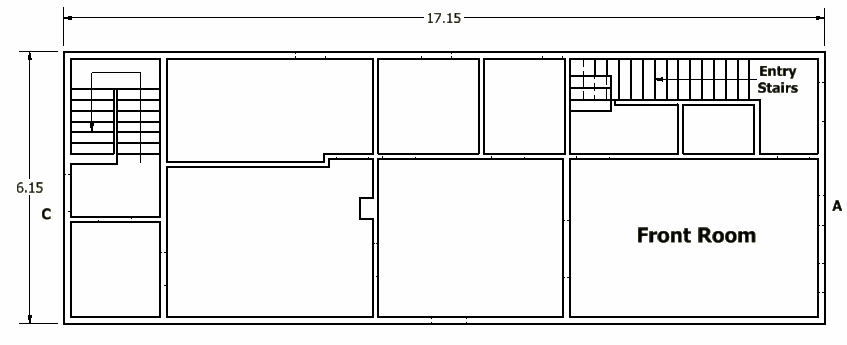
\includegraphics[width=6in]{../Figures/Simple_1_metric} \\
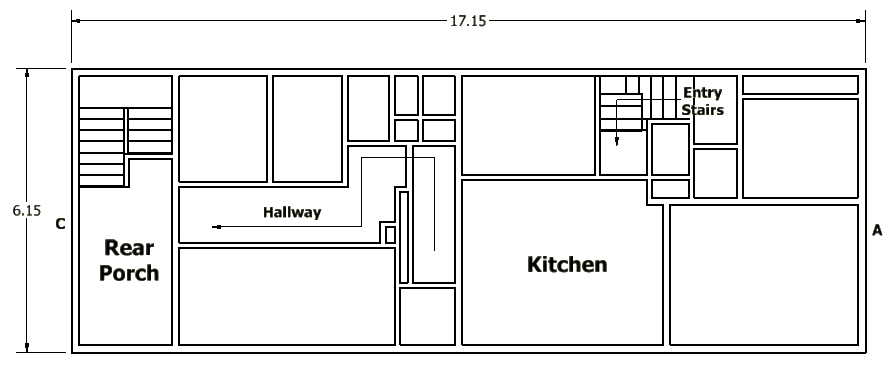
\includegraphics[width=6in]{../Figures/Simple_2_metric}
\end{tabular*}
\caption{Top view of 1st (top) and 2nd (bottom) floor of structure. Stairs and key rooms are identified.}
\label{fig:simp_geom}
\end{figure}

\begin{figure}[h!]
\centering
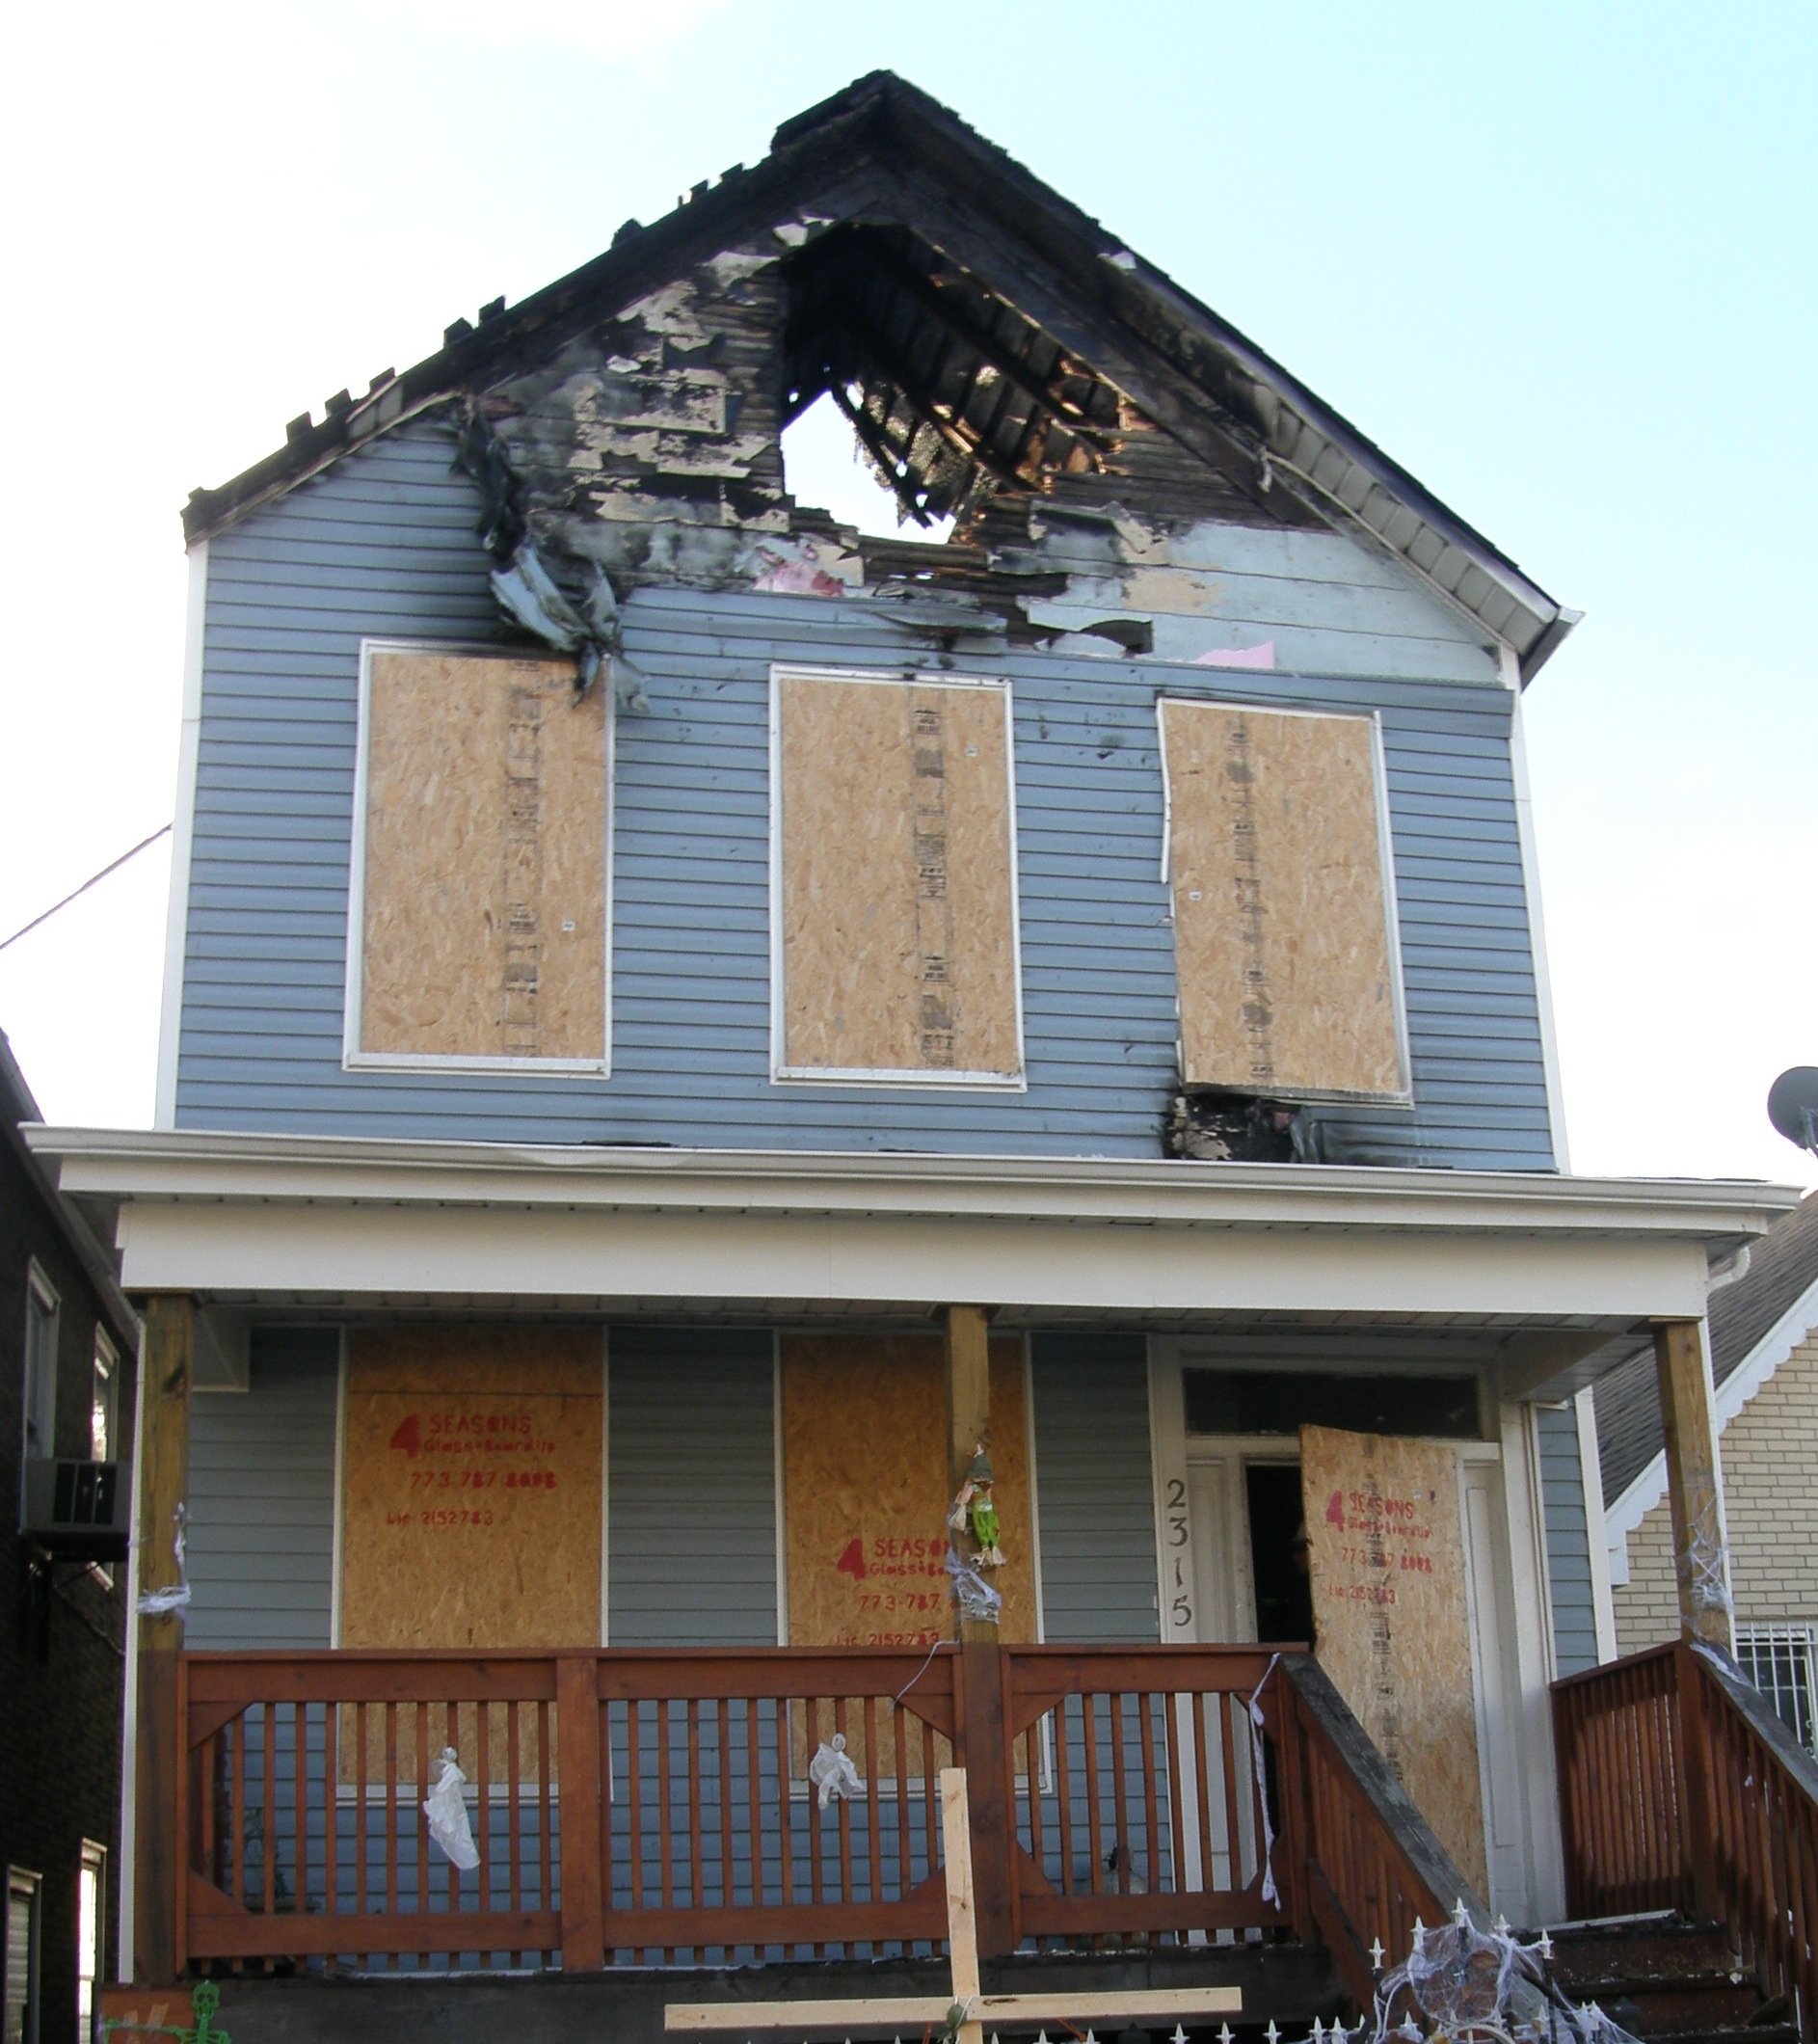
\includegraphics[width=.65\textwidth]{../Figures/exterior_alpha}
\caption{Photograph showing the post-incident front (side alpha) exterior of the structure.}
\label{fig:alpha_ex}
\end{figure}

Figs.~(\ref{fig:first_floor} and \ref{fig:second_floor}) show the interior dimensions of the first and second floor, respectively. The dimensions were found from on-scene measurements using a tape measure. Measurements were made to the nearest 1.27 cm (0.5 in). Based on difficulty of making some of the measurements due to the condition of the post-fire structure, the uncertainty in the measurements is estimated to be on the order of $\pm$ 1 \%. This would result in measurements that could change by up $\pm$ 17 cm ($\approx$ 7 in). When considering the uncertainties in the initial fire development, ventilation (vent times and vent areas), and peak heat release rate among other factors, the uncertainty in the overall structure geometry is not a major factor.

%Fig.~(\ref{fig:smv_interior}) shows 3D Smokeview renderings of cutaways of the beta and delta sides of the structure interior.
%\begin{figure}[h!]
%\begin{tabular*}{\textwidth}{l@{\extracolsep{\fill}}r}
%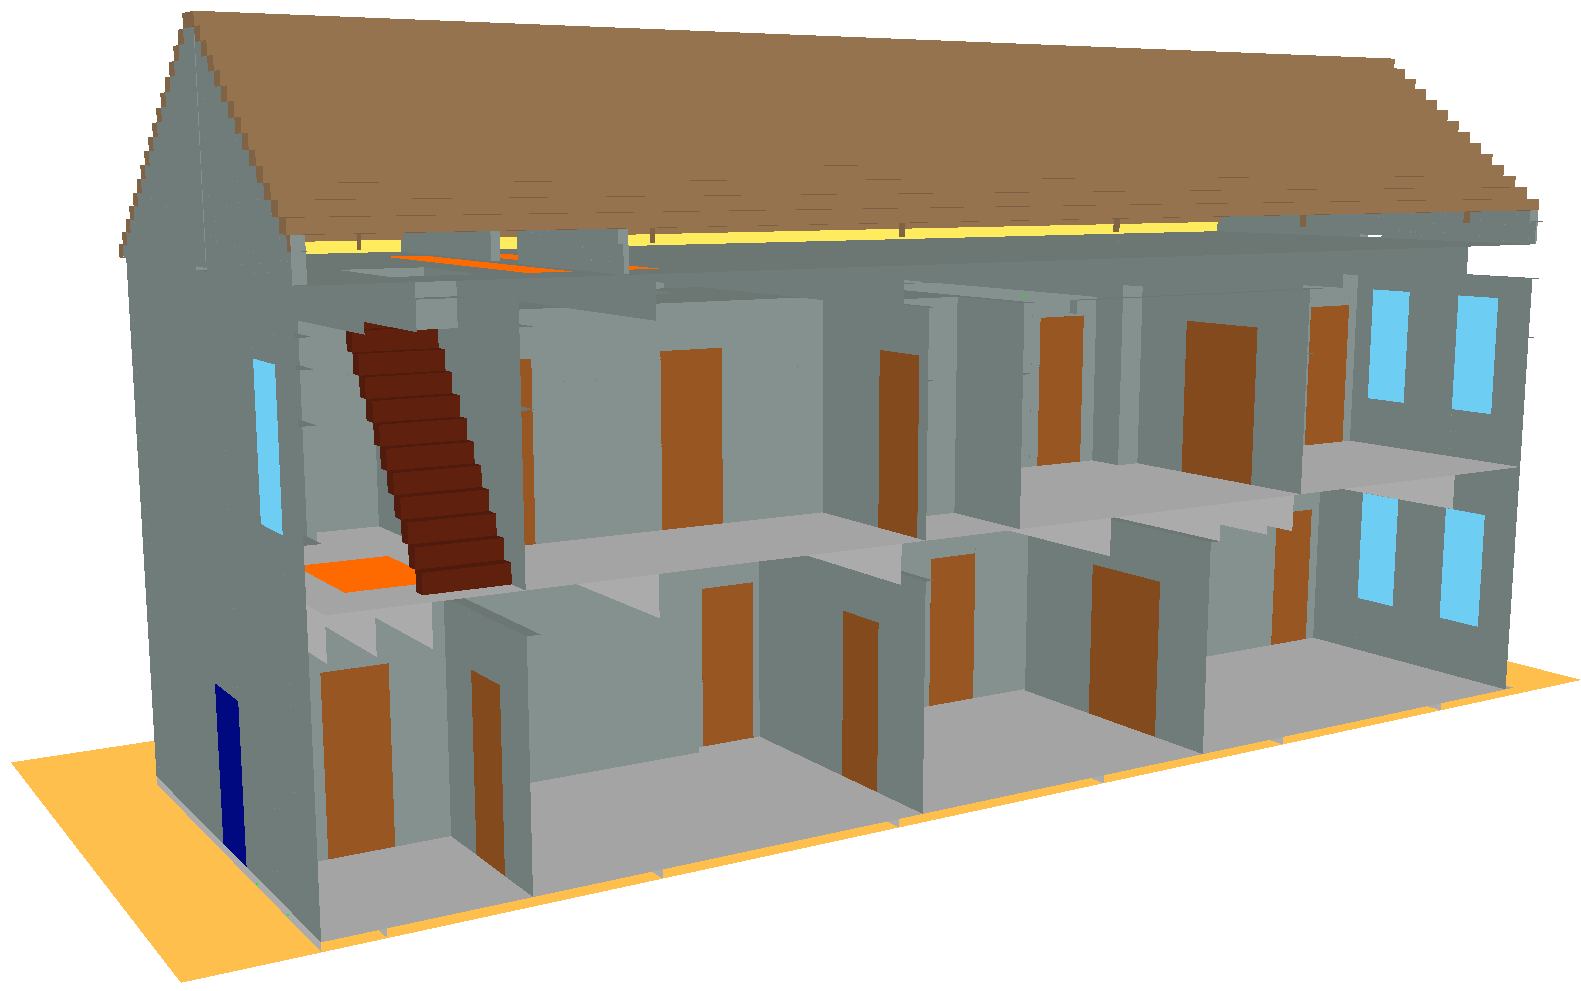
\includegraphics[width=.80\textwidth]{../Figures/interior_beta} \\
%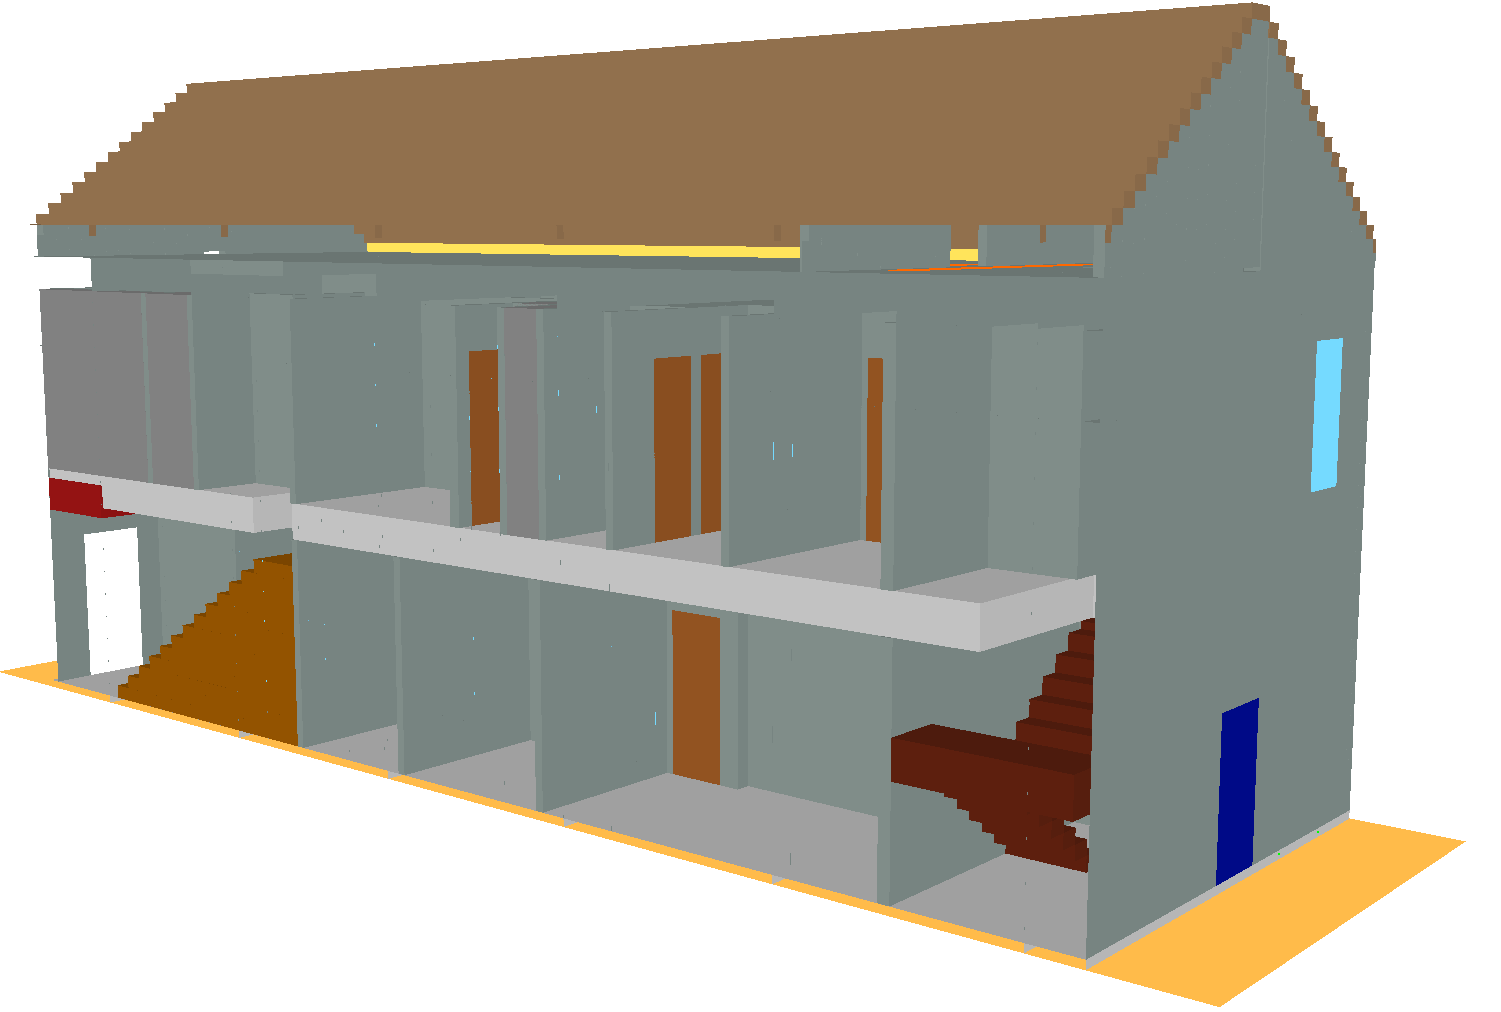
\includegraphics[width=.80\textwidth]{../Figures/interior_delta} \\
%\end{tabular*}
%\caption{3D Smokeview rendering of structure interior looking from the charlie side to both the beta side (top) and to the delta side (bottom)}
%\label{fig:smv_interior}
%\end{figure}


\section{Fire}
\label{fire}

To estimate the fuel, fire size, and structure ventilation, on-scene videos and post-incident reports are used. Post-incident, the fire investigation concluded that the fire originated in the structure's attic~\cite{NIOSH:Bowyer}. Post-fire pictures revealed extensive damage to the attic and second floor rear porch (cf. Fig.~(\ref{fig:charlie_ex})). Based on these findings, the FDS model includes two source fire locations: an initial fire in the attic and a secondary fire on the second floor porch landing. The attic and rear porch consist of a fuel load that is mainly wood: the rear porch was enclosed with wood planks exteriorly covered by foam board and vinyl siding, the roof was asphalt shingles over wood planking, and the attic and porch had oriented strand board (OSB) floors.  

\begin{figure}[h!]
\centering
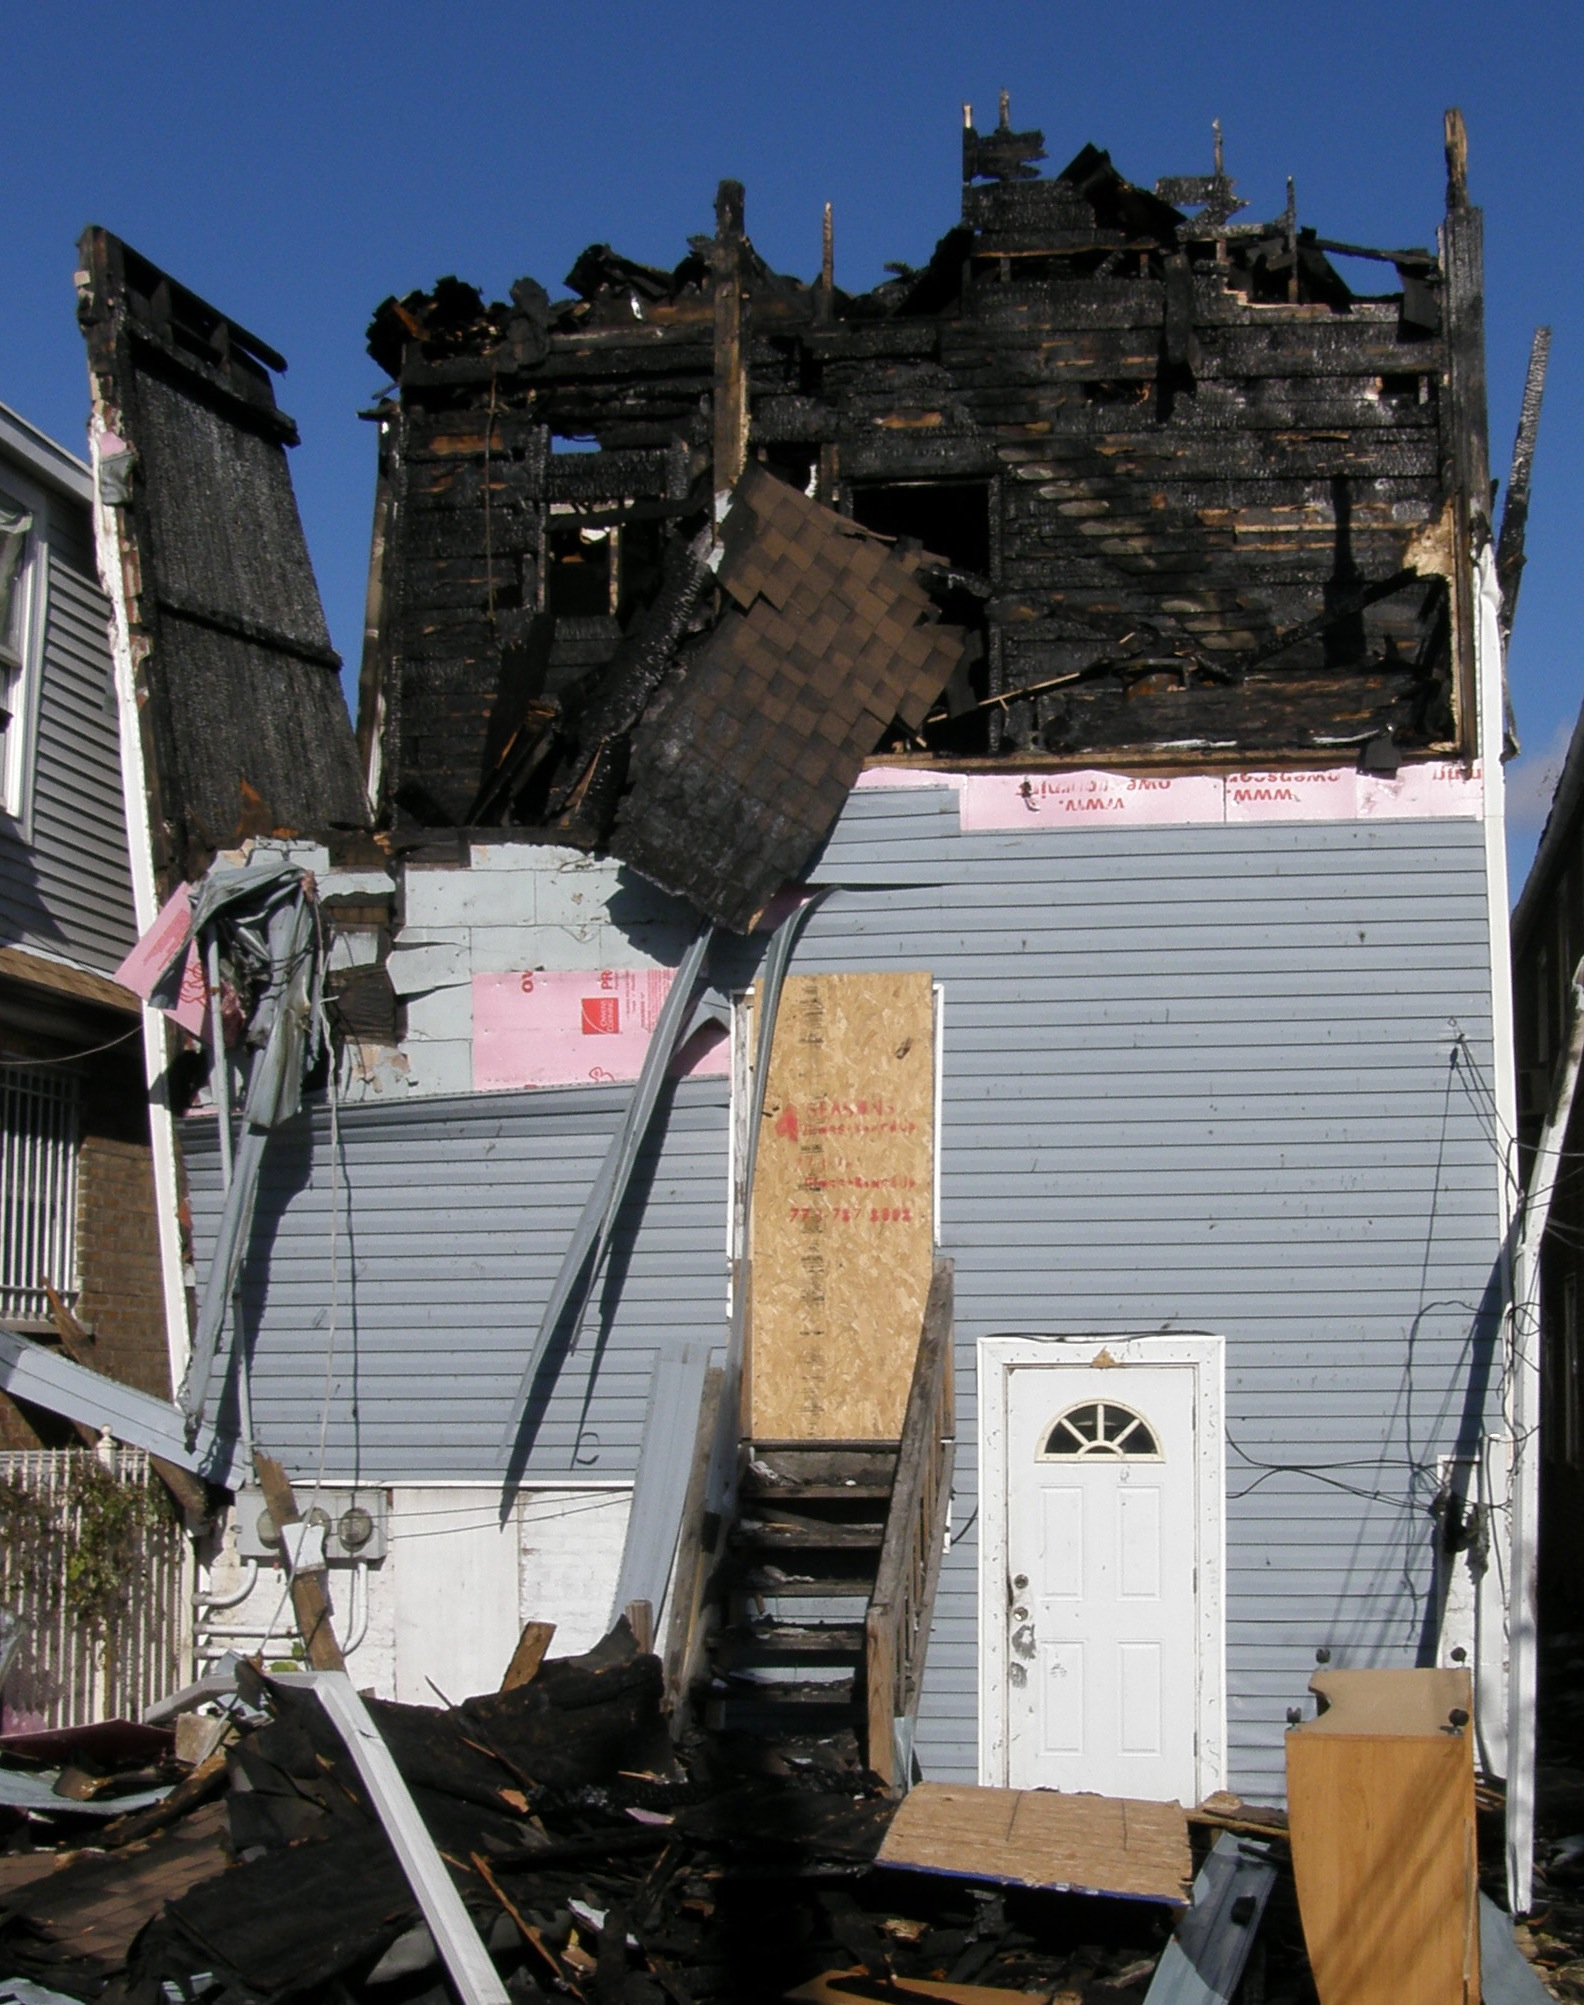
\includegraphics[width=.65\textwidth]{../Figures/exterior_charlie}
\caption{Photograph showing the post-incident rear (side charlie) exterior of the structure.}
\label{fig:charlie_ex}
\end{figure}


If we represent wood with the following chemical formula, $\C\H_{1.7}\O_{0.74}\N_{0.002}$, and use carbon monoxide ($y_{\mathrm{CO}}=0.004 \; {\mathrm{kg_{CO}}/\mathrm{kg_{wood}}}$) and soot ($y_{\mathrm{C}}=0.015 \; {\mathrm{kg_{C}}/\mathrm{kg_{wood}}}$) yields from the SFPE Handbook~\cite{SFPE:Tewarson}, we can write a balanced chemical reaction for wood oxidation:

\begin{multline}
\C\H_{1.7}\O_{0.74}\N_{0.002} + 4.89(0.208\,\O_{2} + 0.783\,\N_{2} + 0.387\text{\sc{e}-}3\,\C\O_{2} + 0.834\text{\sc{e}-}2\,\H_{2}\O) \\ 
\rightarrow 5.84(0.719\text{\sc{e}-}3\,\C\O + 0.168\,\C\O_{2} + 0.155\,\H_{2}\O + 0.669\,\N_{2} + 0.693\text{\sc{e}-}2\,\C)
\label{eq:wood_comb}
\end{multline}

The heat of combustion of wood used in this simulation is 16400 kJ/kg (7050 BTU/lb), based on data provided in the SFPE Handbook~\cite{SFPE:Tewarson}. The heat of combustion quantifies the energy release per unit mass of the fuel. The following text defines Eq.~\ref{eq:wood_comb} for an FDS input file with the desired fuel and reaction properties discussed above:

\begin{lstlisting}
&SPEC ID = 'WOOD', FORMULA = 'CH1.7O0.74N0.002' /

&REAC ID = 'wood' 
    FUEL = 'WOOD', 
    HEAT_OF_COMBUSTION=16400,
    SOOT_YIELD = 0.015,
    CO_YIELD = 0.004/
\end{lstlisting}

Note that using the input lines above will invoke the simple chemistry reaction balance in FDS. This means that fuel and air react to form only CO$_2$, CO, H$_2$O, Soot, and N$_2$. If there is a desire for any other combustion products then the user must explicitly define those species and the chemical reaction that produces them~\cite{FDS_Users_Guide}. Based on above input lines FDS uses the default, mixing-controlled fast chemistry combustion model. This mechanism  states that the rate of fuel consumption is proportional to both the local limiting reactant concentration and the local rate of mixing and extinction is based on the critical flame temperature approach~\cite{FDS_Math_Guide}. While FDS provides users to the option to use a more complex finite-rate combustion mechanism, we do not have sufficient evidence to justify deviating from the default specifications. 

To estimate the energy release per unit time and unit area (kW/m$^2$) of wood, we use work by Babrauskas and Grayson~\cite{babrauskas1990}. Experiments were conducted in a cone calorimeter to determine the 5 minute average of HRRPUA (kW/m$^2$) for several different types of wood over a range of radiant heat fluxes (kW/m$^2$). Here, we take a conservative approach and assume the burning wood in the structure had the lowest energy density of the tested samples~\cite{babrauskas1990}, similar to that of Douglas Fir plywood. Based on the range of heat flux exposures, the data was fit to determine HRRPUA ($y$) as a function of exposure ($x$):

\begin{equation}
y = ax+b
\label{eq:heat_flux}
\end{equation}

In Eq.~\ref{eq:heat_flux}, $a$ and $b$ are experimental constants. For Douglas Fir plywood these values were found to be 1.43 and 22 respectively. Typically radiative feedback from flaming combustion is between 20 kW/m$^2$ and 35 kW/m$^2$~\cite{tsaidrysdale}. If we estimate that the average radiation feedback to the pyrolyzing fuel is 20 kW/m$^2$ because of under-ventilated conditions within the structure, then following Eq.~\ref{eq:heat_flux} the average heat release per unit area (HRRPUA) for wood is 51 kW/m$^2$.

To calculate the total fire size, we need to determine the appropriate burnable area (exposed wood area) of the attic and second floor porch enclosure. Based on the floor plan of the structure, the underside of the roof is approximately 134 m$^2$ (1453 ft$^2$) plus there is 105 m$^2$ (1130 ft$^2$) of floor area in the attic. Examination of post incident images showed that the floor immediately over the back porch burned away. That area will be considered as part of the porch fire. Based on post-incident damage, we consider approximately 50 \% of the remaining floor area as fuel to the attic fire. To estimate the total attic fire size, we include the underside roof area (134 m$^2$) and the floor area (43 m$^2$ (463 ft$^2$)). Using an HRRPUA of wood of 51 kW/m$^2$, results in a fire size of 9 MW. To estimate the porch fire size, we consider the the four walls of porch enclosure (42 m$^2$) and the floor and ceiling of the porch (24 m$^2$ (258 ft$^2$)). The total area is 64 m$^2$ (689 ft$^2$). Using the same HRRPUA of 51 kW/m$^2$, the fire size on the porch is approximately 3.3 MW. The total fire size for this structure is estimated to be 12.3 MW. Since it is unknown when the fire started relative to notification of a fire or how fast the fire spread, several simplifications are made. First is that the attic fire starts at the beginning of the simulation and ramps up to 9 MW in 10 seconds. The porch fire starts 40 seconds into the simulation and ramps to 3.3 MW in 10 seconds. A ten second ramp to peak was used to prevent sharp velocity changes at the fire boundary condition in FDS. The second is that the sources of the gas phase wood fuel are of fixed area and at fixed locations (2 sources for attic, 1 source for porch). The following lines define the source fires for an FDS input file:

\begin{lstlisting}
&SURF ID='FIRE', HRRPUA=2250., COLOR='ORANGE',TAU_Q=10 /
&VENT XB=-13.5,-13,1,5,6.16,6.16, SURF_ID='FIRE' / 2 m^2
&VENT XB=-14.5,-14,1,5,6.16,6.16, SURF_ID='FIRE' / 2 m^2
&VENT XB=-16.5,-15.5,1,2.5,3.14,3.14, SURF_ID='FIRE',DEVC_ID='SECOND FIRE'/ 1.5 m^2
&DEVC XYZ = -17.2,2,0 ID = 'SECOND FIRE', QUANTITY = 'TIME', SETPOINT = 40, INITIAL_STATE = .FALSE. /
\end{lstlisting}
Note that the coordinates here are unique for the vents are specific to the input files used for these simulations. The key point is that they are 2-D planes of a specific area.

\section{Materials}
\label{matl}
While the fire was simplified to constant area fuel sources (Section~\ref{fire}), defining the material properties of the walls and ceiling are still important from a heat transfer perspective. In this study, we define gypsum~\cite{Quintiere:2} for the finished walls and ceilings on the main two floors of the structure and wood~\cite{Incropera:1} for the unfinished portions of the attic and rear porch. The text provided below are the lines necessary to define these materials in an FDS input file.

\begin{lstlisting}
&MATL ID        = 'GYPSUM'
    FYI = 'Quintiere, Fire Behavior' 
    CONDUCTIVITY    = 0.48
    SPECIFIC_HEAT   = 0.84
    DENSITY = 1440./

&MATL ID        = 'WOOD_MAT'
    FYI = 'Incropera and DeWitt, Fundamentals of Heat and Mass Transfer'
    CONDUCTIVITY    = 0.12
    SPECIFIC_HEAT   = 1.38
    DENSITY = 510./ 
\end{lstlisting}

\section{Vents}
\label{Vents}
This simulation includes vents that account for the changes in ventilation due to a combination of fire department operations (opening doors) and fire acting on the structure (fire breaching walls, breaking windows, etc). There are two ventilation scenarios that are considered in this study. The first is the baseline simulation where the ventilation times and ventilation areas represent our best understanding of the incident. The alternative simulation does not include the firefighter opening the rear door to make entry to the structure and the subsequent beta side wall breach. The times of the ventilation changes are provided in Table \ref{tab:vents}. Structure leakage has been shown to be important when modeling enclosure fires~\cite{beal2009}. The open front door at the start of the simulation and the vents (opening size and open time) created during the simulation are significantly larger than the total effective area of leakage of structure of this type. Therefore, leakage would have a negligible impact on the fluid mechanics within the structure and is not included in this study.

\begin{table}
\centering
\captionof{table}{Simulation Ventilation Timelines}\label{tab:vents}
\begin{tabular}{ccccc}
\toprule[1.5pt]
Baseline Simulation & Alternative Simulation & Ventilation Area [m$^2$] & Type & Structure Side \\
\midrule
00    &  00   & 0.11 & Window      & Charlie \\
40    &  40   & 0.08 & Breach (x2) & Alpha and Charlie \\
45    &  45   & 0.12 & Breach      & Beta \\
55    &  55   & 0.12 & Breach      & Charlie \\     
130   &  N/A  & 1.41 & Door        & Charlie \\
135   &  N/A  & 0.2  & Breach      & Beta \\        
160   &  160  & 0.80 & Door        & Interior \\
\bottomrule[1.25pt]
\end{tabular}\par
\end{table}

\section{Mesh}
\label{mesh}

For the simulation in this study, we can estimate a measure of how well the flow field is resolved by the non-dimensional expression $D^*/\dx$. Here $D^*$ is a characteristic fire diameter, $\dx$ is the nominal size of a mesh cell, and $\dQ$ is the total heat release rate of the fire:
\begin{equation}
D^* = \left(
     \frac{\dQ}{\rho_\infty \, c_p \, T_\infty \, \sqrt{g} }
     \right)^\frac{2}{5} 
\label{eq:mesh}
\end{equation}   
From the FDS User Guide~\cite{FDS_Users_Guide}, ``the characteristic fire diameter is related to the characteristic fire size via the
relation $Q^* = (D^*/D)^{5/2}$.'' Here, $D$ is the physical diameter of the fire as input to the model. Following Eq.~(\ref{eq:mesh}) and using 10 cm grid cells, the characteristic fire diameter to cell size ratio based on the 3.3 MW porch fire is 15.5 and for the 9 MW fire is 23. Based on validation work performed for the U.S. Nuclear Regulatory Commission, $D^*/\dx$ values ranged between 4 and 1~\cite{NUREG_1824}. The grid resolution used in the model falls within typical, engineering $D^*/\dx$ values. As a result, all of the input model geometry lengths, ventilation openings (holes, doors, and windows), and fire areas will snap to the nearest 10 cm. Fig.~(\ref{fig:geom_grid}) shows the 
alpha side (front) of the structure rendered in Smokeview with the 10 cm mesh.

\begin{figure}[h!]
\centering
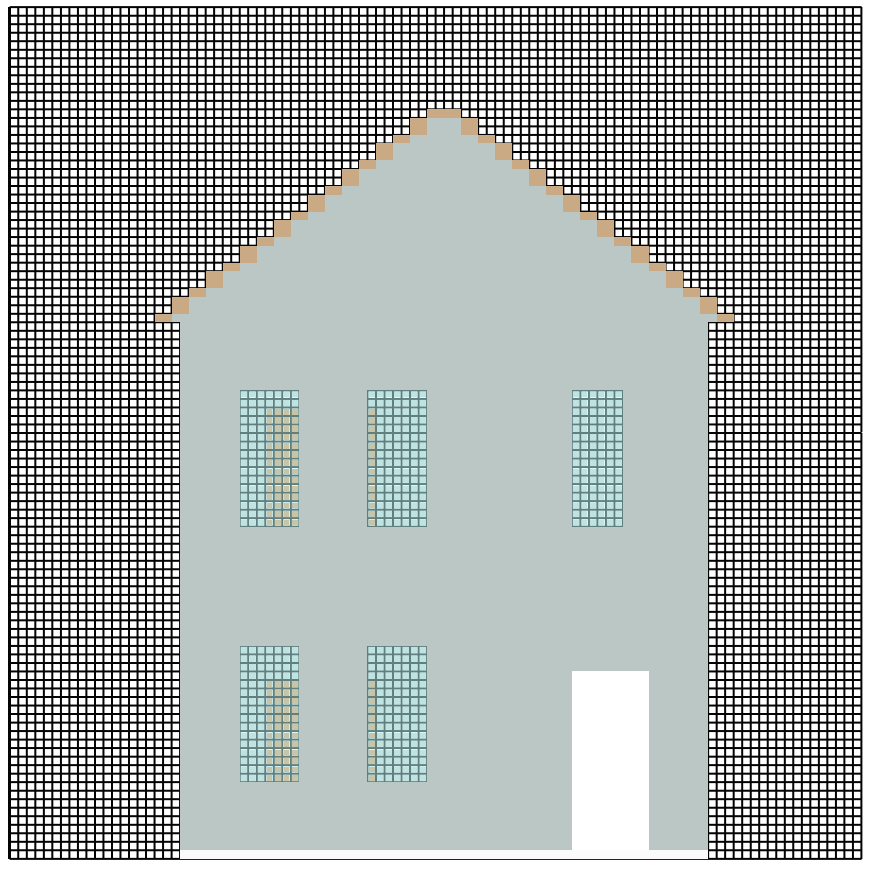
\includegraphics[width=.60\textwidth]{../Figures/smv_exterior_grid}
\caption{Alpha side of the structure with 10 cm computation mesh.}
\label{fig:geom_grid}
\end{figure}

As discussed Section~\ref{geom}, the structure has 17.15 m (56 ft) by 6.15 m (20ft) footprint with a total height of 8.56 m (28 ft). To ensure adequately resolved fluid flow into and out of the structure the computational domain is extended beyond the volume of the structure. The total volume of the computational domain is 24 m (79 ft) by 10 m (33 ft) by 10 m (33 ft). At 10 cm (3.9 in) resolution this would result in 2.4 million computational cells. To make the simulation time more tractable, the domain was divided into 16 equal 150 thousand cell meshes to be processed in parallel. Fig.~(\ref{fig:mult_mesh}) shows the entire structure within the computational domain.

\begin{figure}[h!]
\centering
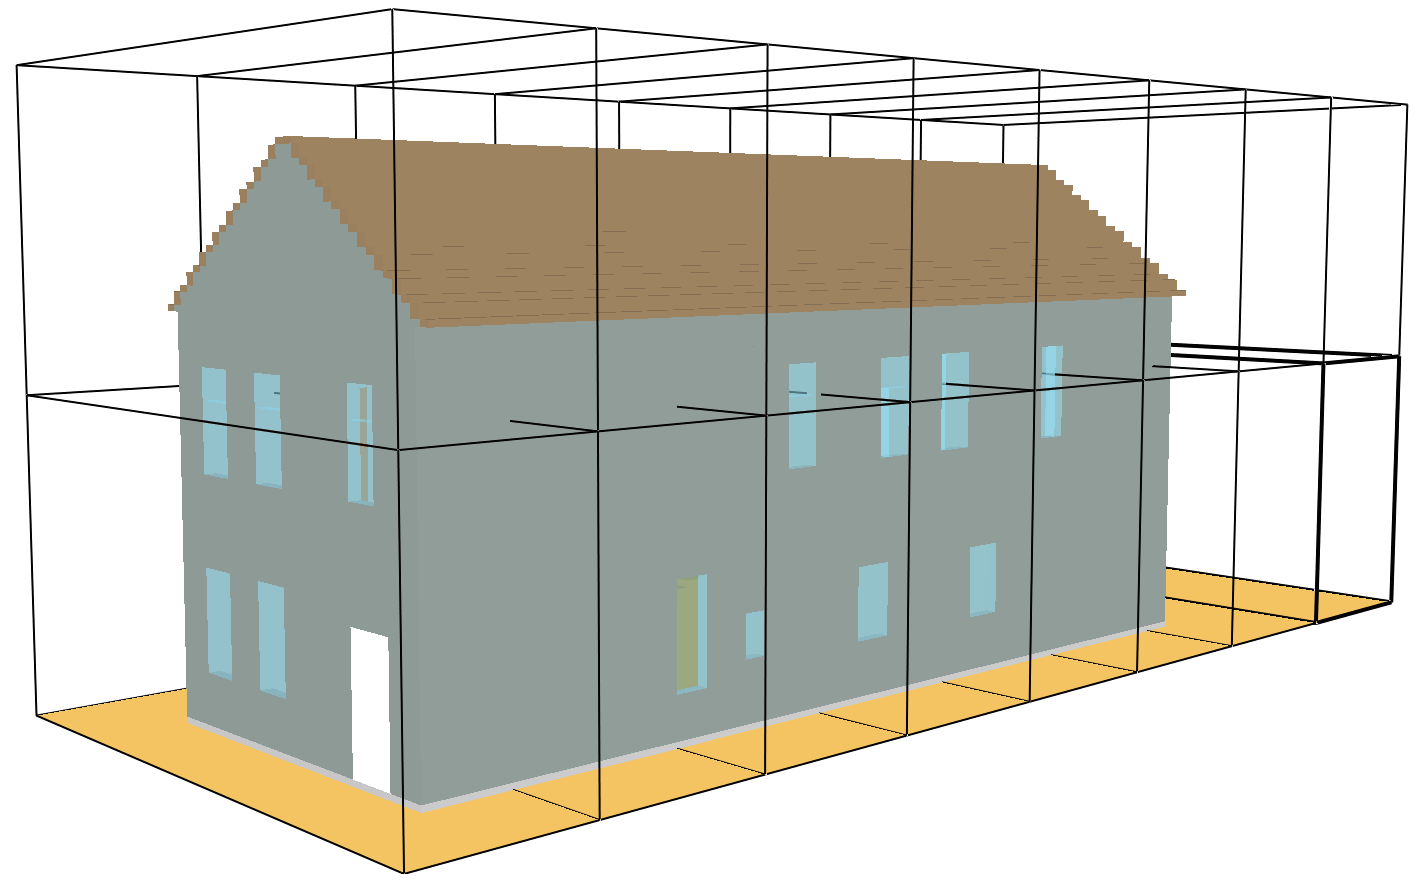
\includegraphics[width=.60\textwidth]{../Figures/smv_exterior_mesh}
\caption{Alpha-Delta side of the structure within computational domain. Each of the 16 meshes is 3 m (9.8 ft) by 10 m (33 ft) by 5 m (16.4 ft).}
\label{fig:mult_mesh}
\end{figure}

\chapter{Model Results}
\label{results}

\section{Heat Release Rate}
\label{HRR}
The heat release rate output data from FDS quantifies the model-predicted rate of energy release in the simulation. Here, we examine impact of ventilation on fire size. Fig.~(\ref{fig:hrr}) shows the HRR versus time based on the prescribed fires described in Section \ref{fire} and the FDS results for two venting scenarios. The two vertical lines represent when a firefighter opened the back door of the structure (t = 130 s) and when the second floor interior door was estimated to fail (t = 160 s).

\begin{figure}[h!]
\centering
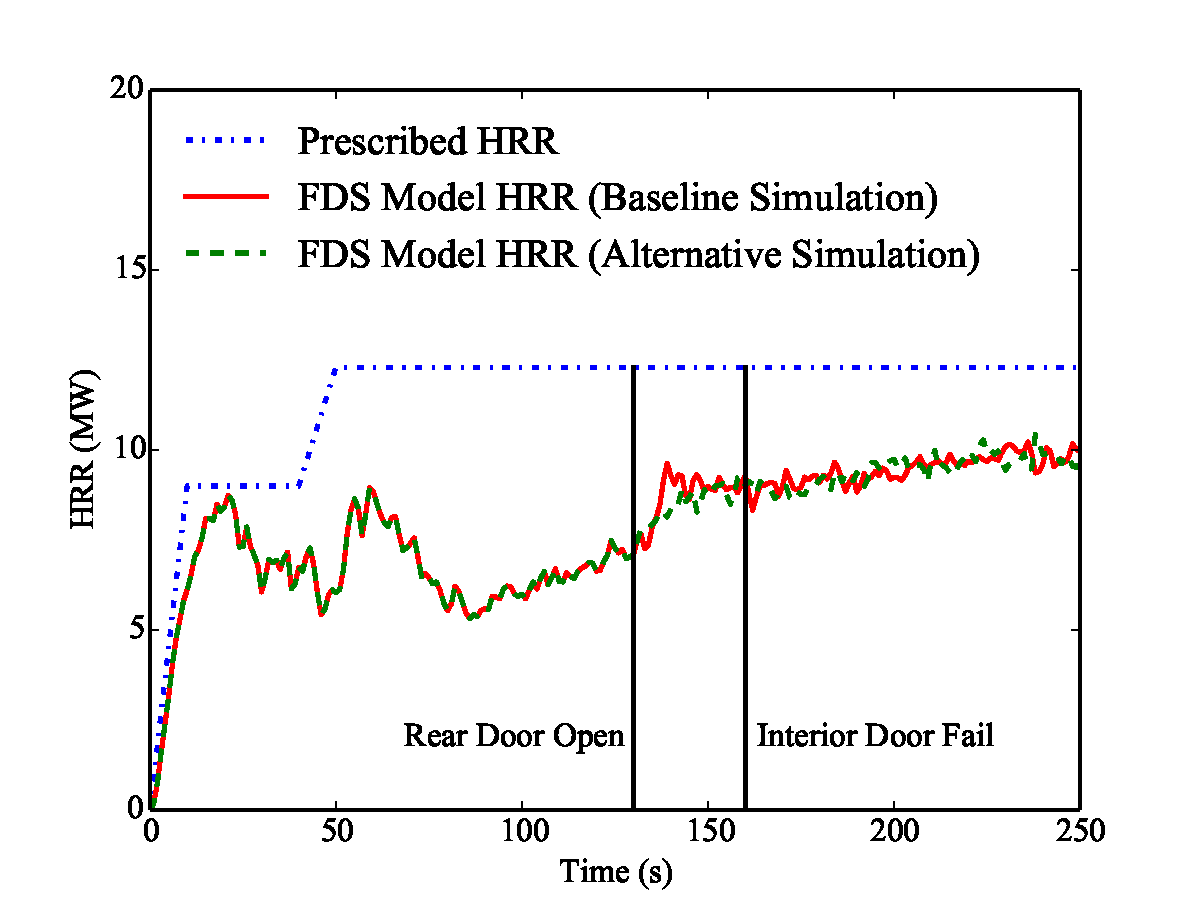
\includegraphics[width=.80\textwidth]{../Figures/Chicago_Fire_HRR}
\caption{HRR versus time of FDS model of the West 50th St. fire. The first vertical line indicates when the back door failed, the second indicates when the interior hallway door failed.}
\label{fig:hrr}
\end{figure}

In Fig.~(\ref{fig:hrr}), the solid line is the baseline FDS simulation (this represents the on-scene conditions). The dashed line represents an alternative series events, specifically the rear door does not get opened and the subsequent beta side breach does not occur. The dash-dotted line is the prescribed FDS input HRR. We can see that within the first 10 seconds, the structure is under-ventilated as the modeled HRR is below the prescribed HRR. The HRR peaks at just under 9 MW (approximately 20 seconds into the simulation) before becoming oxygen limited. The HRR drops to 5 MW as the available oxygen inside the structure gets consumed. There is insufficient available oxygen in the structure to combust all of the fuel and combustion occurs locally at vents. Fig.~(\ref{fig:smv_ext_fire}) illustrates exterior flaming combustion through the failed Charlie side window and attic breach just after the second fire ignites at 40 seconds. After additional wall breaches at 45 and 55 seconds (see Table~\ref{tab:vents}), the abrupt change in ventilation causes the HRR spikes to 9 MW before again dropping to about 6 MW. The HRR then begins to increase towards a sustainable steady state value.

From Fig.~(\ref{fig:hrr}), we see that the HRR for both FDS simulations are identical until 130 seconds (HRR $\approx$ 7 MW). At 130 seconds the rear door is opened in the baseline simulation. At 135 seconds there is an additional beta side breach (Table~\ref{tab:vents}). The open door and breach act as additional pressure releases for the structure. Again, the abrupt change in ventilation causes the HRR to spike. Here we see a rise from 7 MW to 9.7 MW at 139 seconds. At the time of door failure (160 seconds), the HRR in both cases was approximately 9 MW as there was sufficient ventilation. While there might be some locally different burning characteristics between the baseline simulation and the alternate simulation, in both cases the interior conditions represented a significant hazard to firefighters inside the structure. Therefore, the analysis will focus on the results of the baseline simulation.

\begin{figure}[h!]
\centering
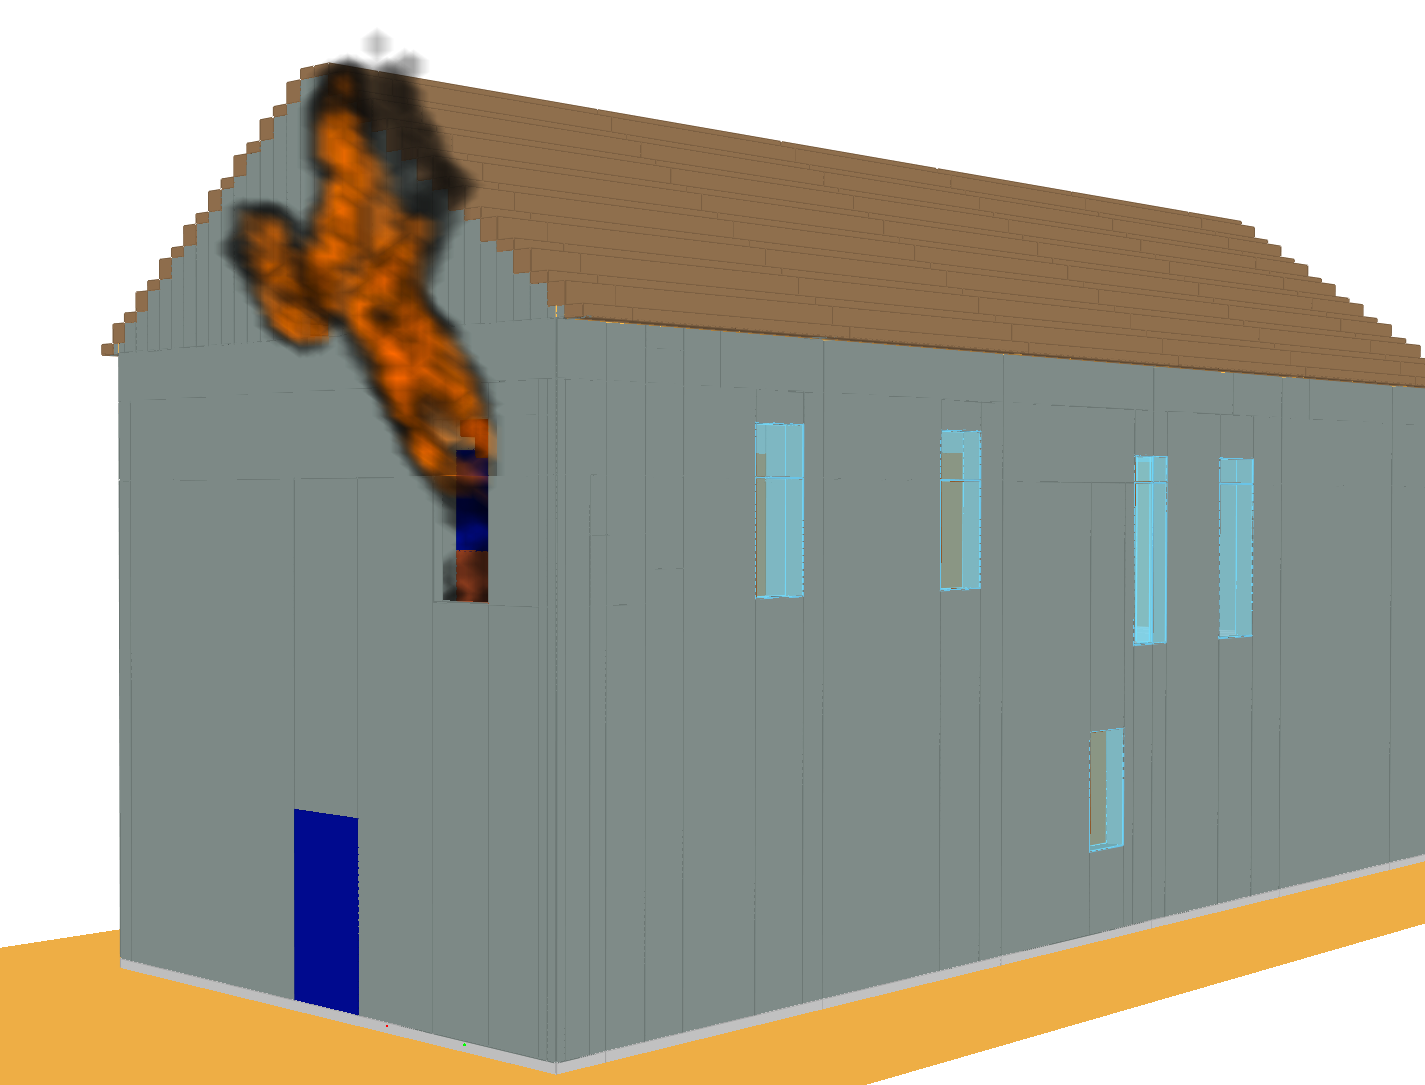
\includegraphics[width=.675\textwidth]{../Figures/smv_exterior_fire}
\caption{Smokeview rendering showing combustion occurring exterior to the structure on the Charlie side.}
\label{fig:smv_ext_fire}
\end{figure}

\section{Pressure}
As the fire grows in the attic and back porch, the pressure rises. Fig.~(\ref{fig:pres_159s}) shows the pressure rise in the structure just before the interior door failed in the simulation. On the rear porch, the pressure rise ranges from a 4 Pa over pressure 1 m off the floor to greater than 10 Pa at the ceiling.
\begin{figure}[!ht]
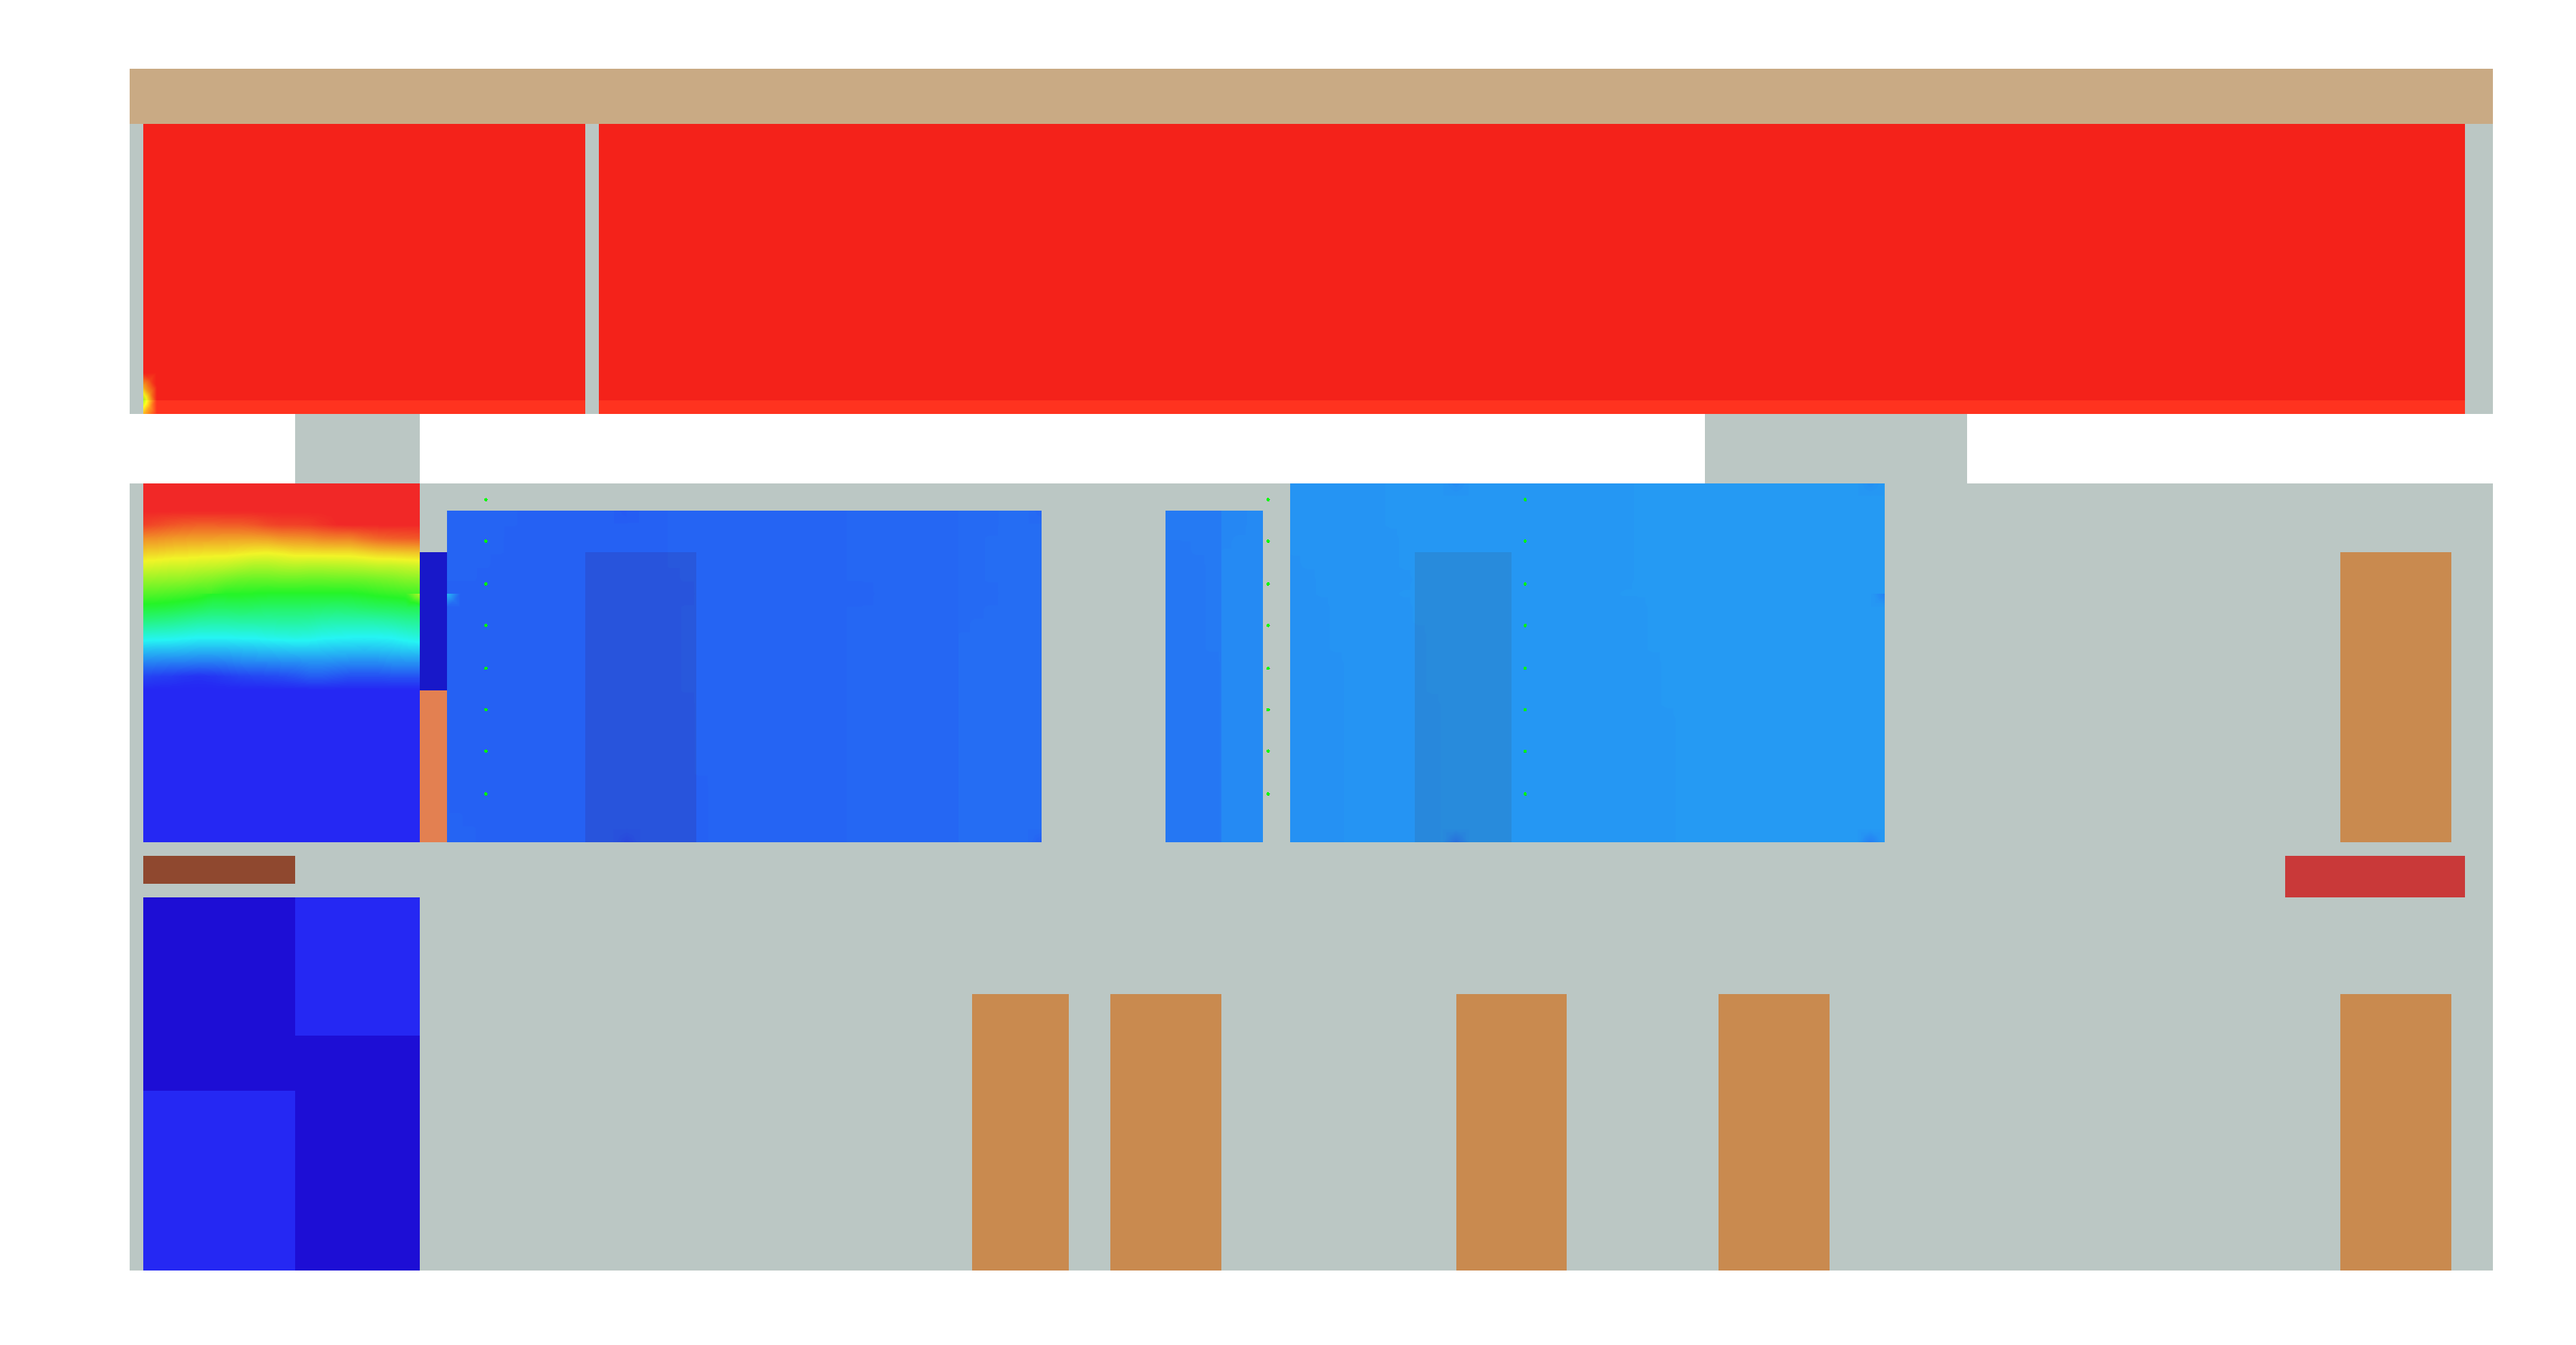
\includegraphics[width=.75\textwidth]{../Figures/west_50th_baseline_pres}
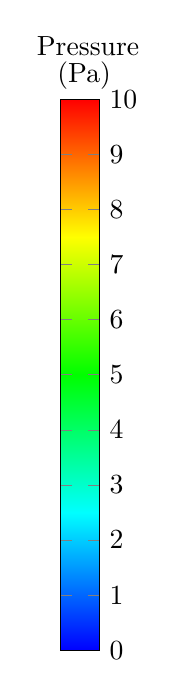
\begin{tikzpicture}
\pgfkeys{/pgf/number format/set thousands separator = {}}
\node at (0.65,0.67) {Pressure};
\node at (0.6,0.3) {(Pa)};
\begin{axis}[
    hide axis,
    scale only axis,
    height=0pt,
    width=0pt,
    colorbar,
    point meta min=0,
    point meta max=10,
    colorbar style={
        height=7cm,
        ytick={0,1,2,...,10}}
    ]
    \addplot [draw=none] coordinates {(0,0)};
\end{axis}
\end{tikzpicture}

\caption{FDS predicted pressure contours, 1 second prior to interior door failure.}
\label{fig:pres_159s}
\end{figure}
 

\section{Temperature}
Analysis of the predicted simulation temperatures will focus on the high hazard areas of the structure: the attic, the rear porch and stairwell, and the interior hallway which connects the rear porch to the front stairwell. Here, we will examine the temperature profile through these high hazards area at several snapshots in time to illustrate the changing interior conditions. The first times are 129 seconds into the simulation, just before a firefighter opened the rear porch door (cf. Fig.~(\ref{fig:temp_129s})) and 159 seconds into the simulation, just before the interior door fails (cf. Fig.~(\ref{fig:temp_159s})).

\begin{figure}[!ht]
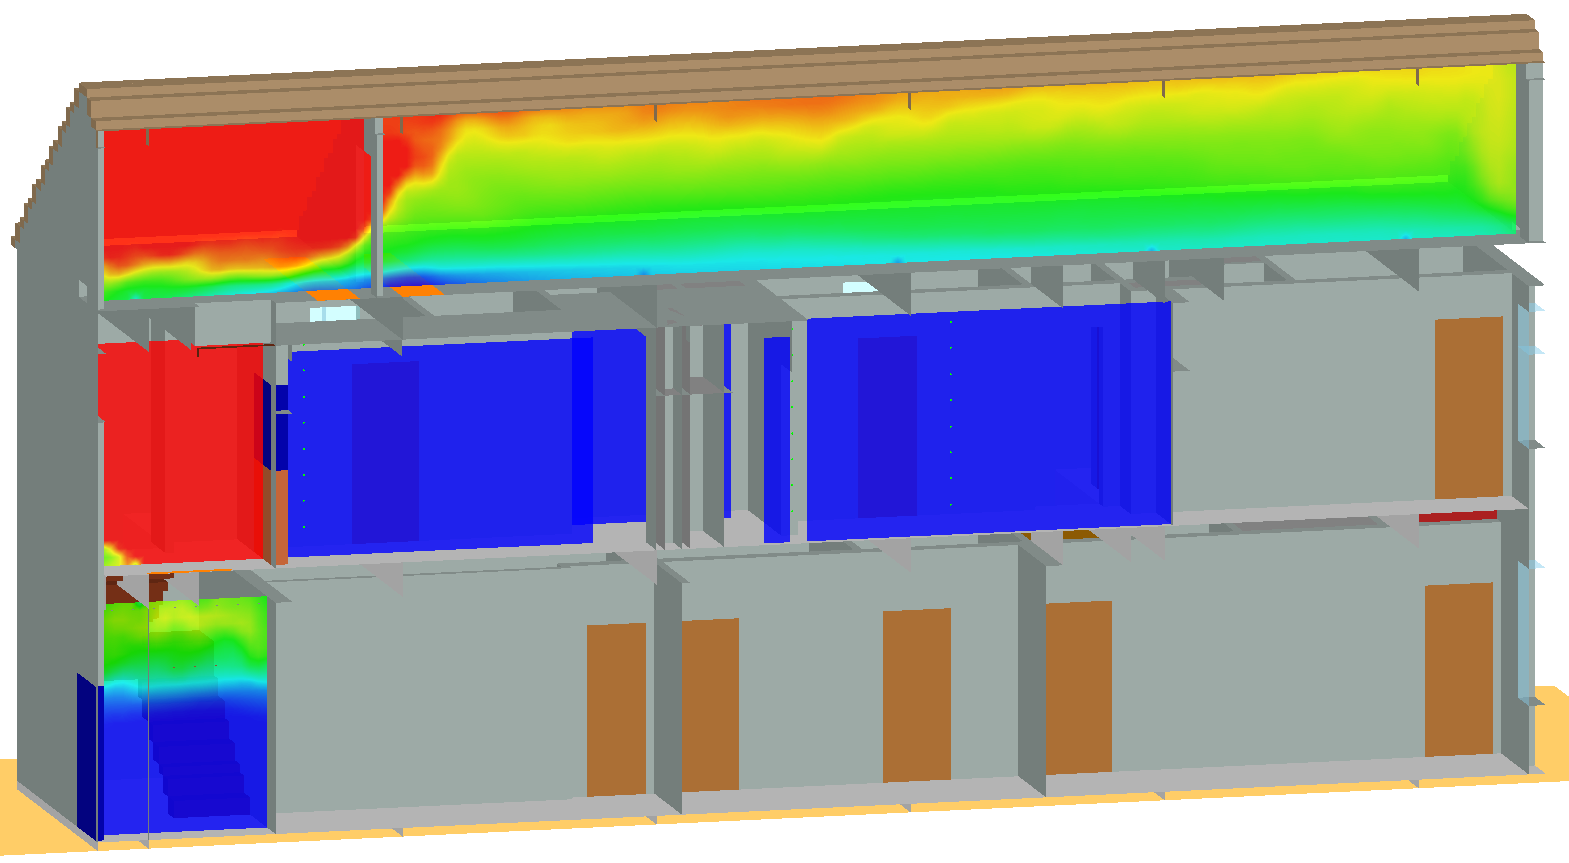
\includegraphics[width=.675\textwidth]{../Figures/west_50th_baseline_129}
%\documentclass{standalone}
%\usepackage{pgfplots}
%\begin{document}
%\pgfplotsset{
%	colormap={blackwhite}{[5pt]
%		rgb255(0pt)=(0,0,255); 
%		rgb255(100pt)=(0,255,255); 
%		rgb255(200pt)=(0,255,0); 
%		rgb255(300pt)=(255,255,0); 
%		rgb255(400pt)=(255,0,0)
%	},
%}
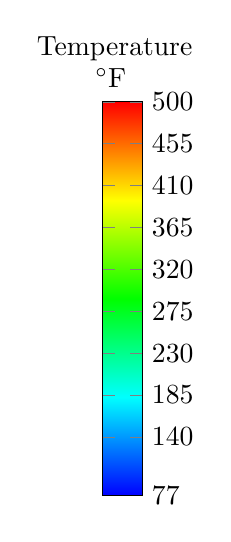
\begin{tikzpicture}
\node at (0.45,0.67) {Temperature};
\node at (0.4,0.3) {$^\circ$F};
\begin{axis}[
    hide axis,
    scale only axis,
    height=0pt,
    width=0pt,
    colorbar,
    point meta min=77,
    point meta max=500,
    colorbar style={
        height=5cm,
        ytick={77,140,185,...,500}
    }]
    \addplot [draw=none] coordinates {(0,0)};
\end{axis}
\end{tikzpicture}
%\end{document} 
%\documentclass{standalone}
%\usepackage{pgfplots}
%\begin{document}
%\pgfplotsset{
%	colormap={blackwhite}{[5pt]
%		rgb255(0pt)=(0,0,255); 
%		rgb255(100pt)=(0,255,255); 
%		rgb255(200pt)=(0,255,0); 
%		rgb255(300pt)=(255,255,0); 
%		rgb255(400pt)=(255,0,0)
%	},
%}
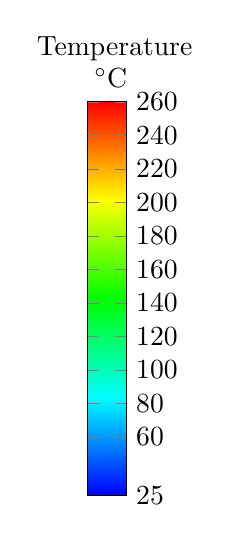
\begin{tikzpicture}
\node at (0.65,0.67) {Temperature};
\node at (0.6,0.3) {$^\circ$C};
\begin{axis}[
    hide axis,
    scale only axis,
    height=0pt,
    width=0pt,
    colorbar,
    point meta min=25,
    point meta max=260,
    colorbar style={
        height=5cm,
        ytick={25,60,80,...,260}
    }]
    \addplot [draw=none] coordinates {(0,0)};
\end{axis}
\end{tikzpicture}
%\end{document}

\caption{FDS predicted temperature contours, 1 second prior to rear door opening.}
\label{fig:temp_129s}
\end{figure}

\begin{figure}[!ht]
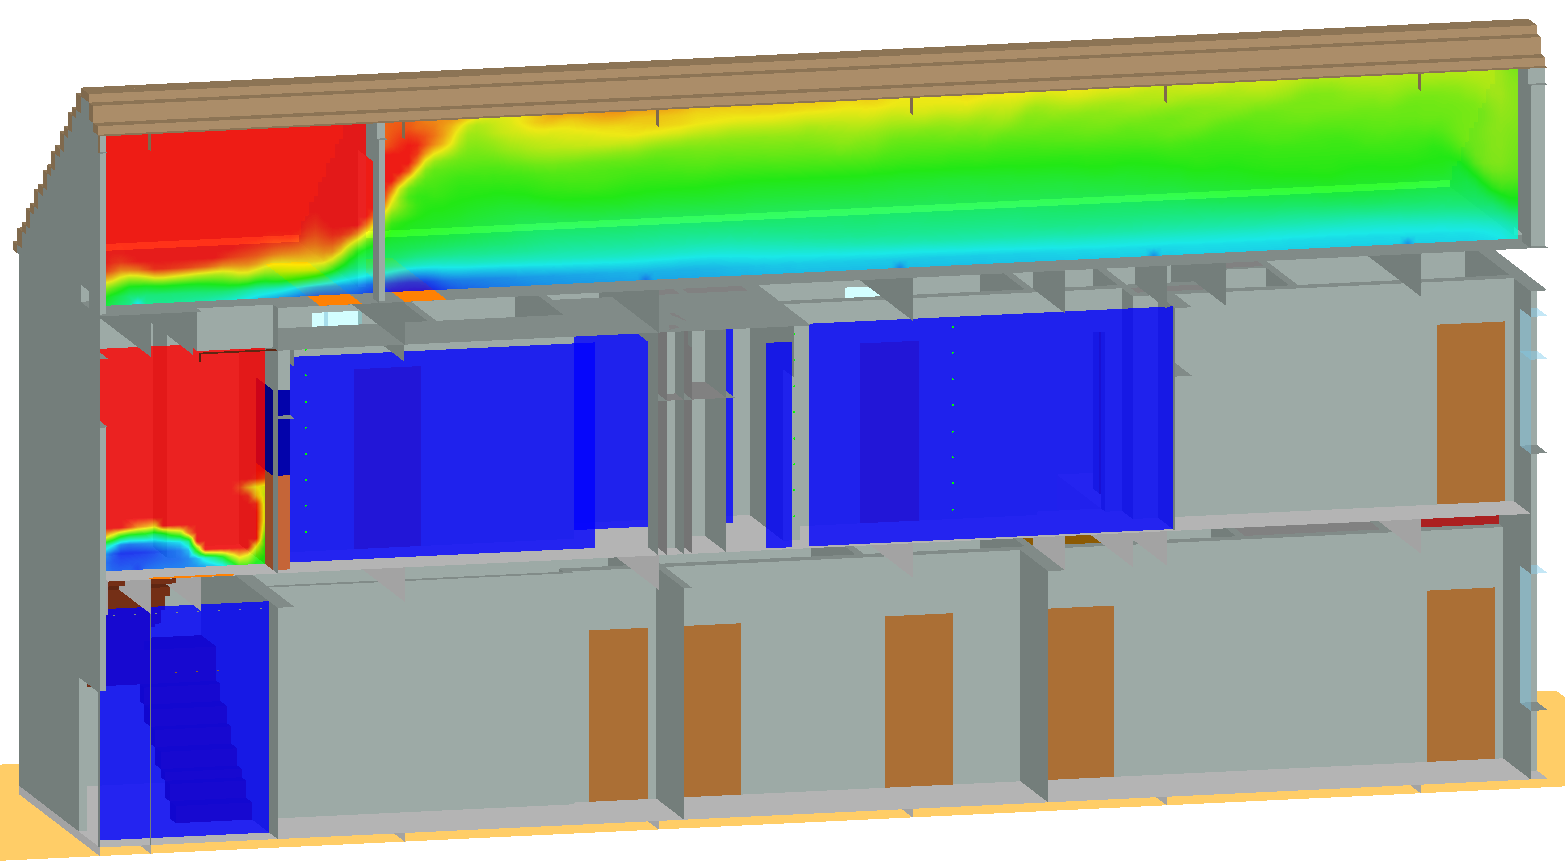
\includegraphics[width=.675\textwidth]{../Figures/west_50th_baseline_159}
%\documentclass{standalone}
%\usepackage{pgfplots}
%\begin{document}
%\pgfplotsset{
%	colormap={blackwhite}{[5pt]
%		rgb255(0pt)=(0,0,255); 
%		rgb255(100pt)=(0,255,255); 
%		rgb255(200pt)=(0,255,0); 
%		rgb255(300pt)=(255,255,0); 
%		rgb255(400pt)=(255,0,0)
%	},
%}
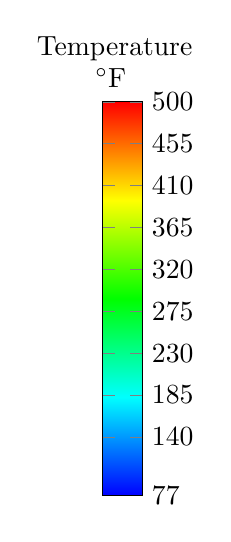
\begin{tikzpicture}
\node at (0.45,0.67) {Temperature};
\node at (0.4,0.3) {$^\circ$F};
\begin{axis}[
    hide axis,
    scale only axis,
    height=0pt,
    width=0pt,
    colorbar,
    point meta min=77,
    point meta max=500,
    colorbar style={
        height=5cm,
        ytick={77,140,185,...,500}
    }]
    \addplot [draw=none] coordinates {(0,0)};
\end{axis}
\end{tikzpicture}
%\end{document} 
%\documentclass{standalone}
%\usepackage{pgfplots}
%\begin{document}
%\pgfplotsset{
%	colormap={blackwhite}{[5pt]
%		rgb255(0pt)=(0,0,255); 
%		rgb255(100pt)=(0,255,255); 
%		rgb255(200pt)=(0,255,0); 
%		rgb255(300pt)=(255,255,0); 
%		rgb255(400pt)=(255,0,0)
%	},
%}
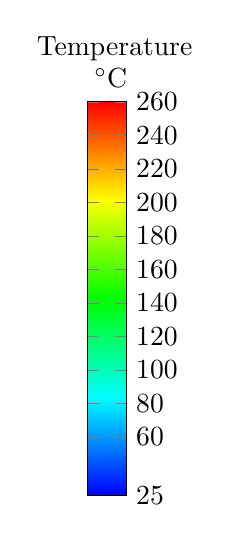
\begin{tikzpicture}
\node at (0.65,0.67) {Temperature};
\node at (0.6,0.3) {$^\circ$C};
\begin{axis}[
    hide axis,
    scale only axis,
    height=0pt,
    width=0pt,
    colorbar,
    point meta min=25,
    point meta max=260,
    colorbar style={
        height=5cm,
        ytick={25,60,80,...,260}
    }]
    \addplot [draw=none] coordinates {(0,0)};
\end{axis}
\end{tikzpicture}
%\end{document}

\caption{FDS predicted temperature contours, 1 second prior to interior door failure.}
\label{fig:temp_159s}
\end{figure}

Fig.~(\ref{fig:temp_129s}) shows temperatures of at least 260 $^{\circ}$C (500 $^{\circ}$F) in the second floor rear porch and rear portion of the attic. High temperatures, between 80 $^{\circ}$C (185 $^{\circ}$F) and 200 $^{\circ}$C (390 $^{\circ}$F), also extend down to the 1$^{st}$ floor rear entrance. Before the interior door fails, Fig.~(\ref{fig:temp_159s}), the inflow ambient air from the open door lowers the temperature local to the doorway, but we know from Fig.~(\ref{fig:hrr}) that over this interval the HRR spikes because of the additional ventilation. After the second floor door fails, (cf. Fig.~(\ref{fig:temp_161s})), the high temperature gas that filled the back porch flows in the direction of lower pressure (towards the front door). Note that the conditions in the attic do not seem to be influenced.
\begin{figure}[!ht]
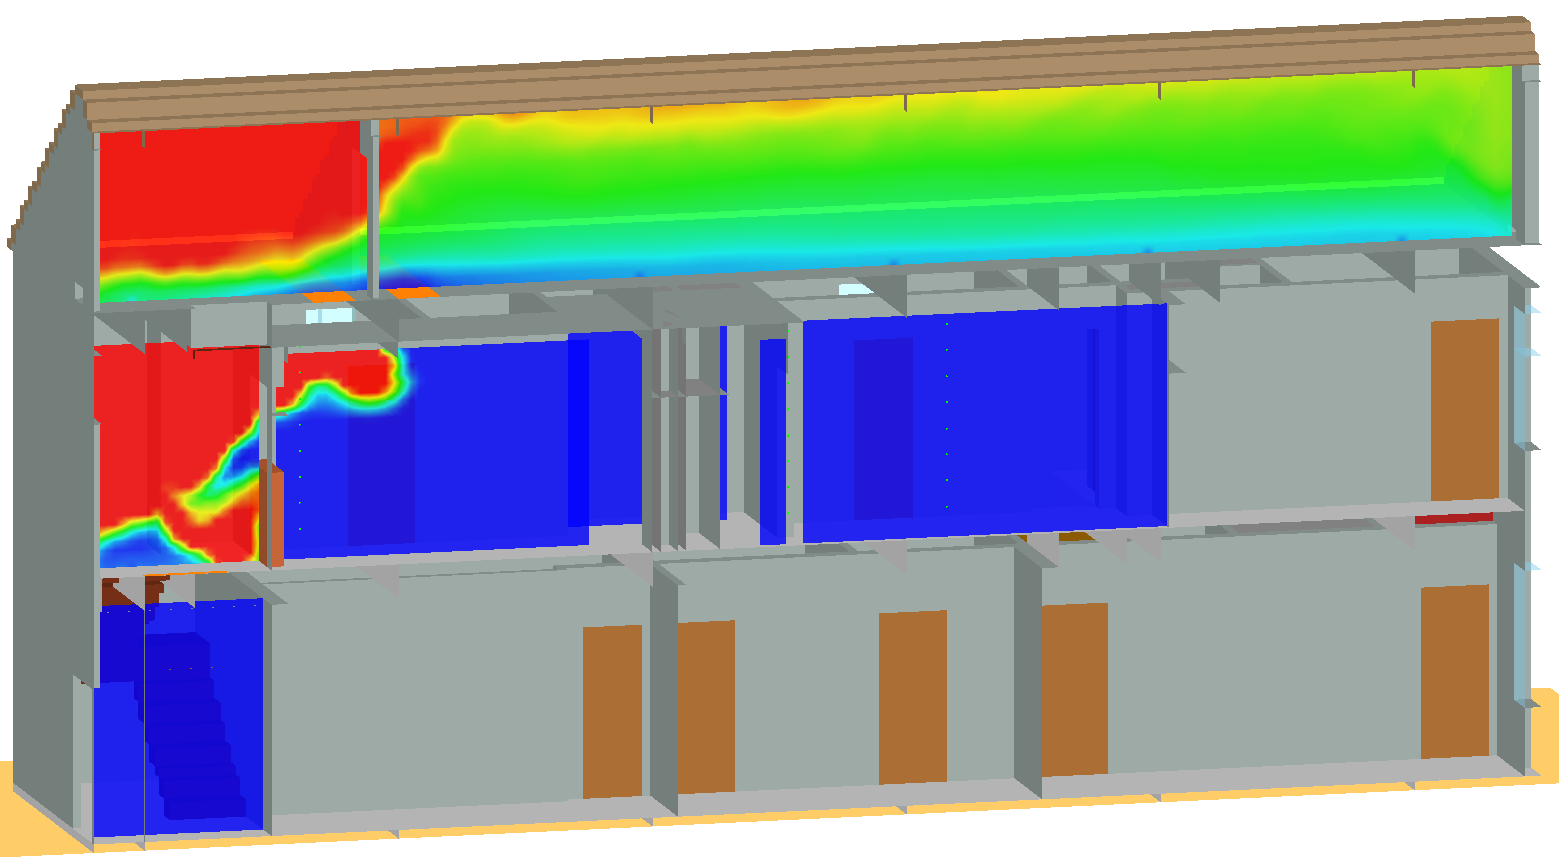
\includegraphics[width=.675\textwidth]{../Figures/west_50th_baseline_161}
%\documentclass{standalone}
%\usepackage{pgfplots}
%\begin{document}
%\pgfplotsset{
%	colormap={blackwhite}{[5pt]
%		rgb255(0pt)=(0,0,255); 
%		rgb255(100pt)=(0,255,255); 
%		rgb255(200pt)=(0,255,0); 
%		rgb255(300pt)=(255,255,0); 
%		rgb255(400pt)=(255,0,0)
%	},
%}
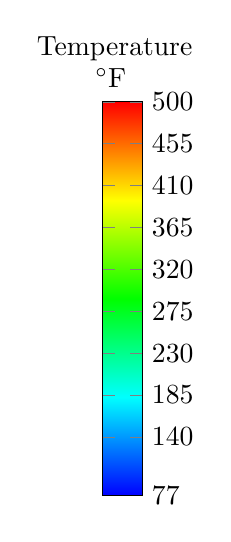
\begin{tikzpicture}
\node at (0.45,0.67) {Temperature};
\node at (0.4,0.3) {$^\circ$F};
\begin{axis}[
    hide axis,
    scale only axis,
    height=0pt,
    width=0pt,
    colorbar,
    point meta min=77,
    point meta max=500,
    colorbar style={
        height=5cm,
        ytick={77,140,185,...,500}
    }]
    \addplot [draw=none] coordinates {(0,0)};
\end{axis}
\end{tikzpicture}
%\end{document} 
%\documentclass{standalone}
%\usepackage{pgfplots}
%\begin{document}
%\pgfplotsset{
%	colormap={blackwhite}{[5pt]
%		rgb255(0pt)=(0,0,255); 
%		rgb255(100pt)=(0,255,255); 
%		rgb255(200pt)=(0,255,0); 
%		rgb255(300pt)=(255,255,0); 
%		rgb255(400pt)=(255,0,0)
%	},
%}
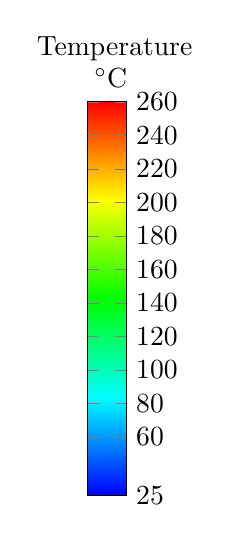
\begin{tikzpicture}
\node at (0.65,0.67) {Temperature};
\node at (0.6,0.3) {$^\circ$C};
\begin{axis}[
    hide axis,
    scale only axis,
    height=0pt,
    width=0pt,
    colorbar,
    point meta min=25,
    point meta max=260,
    colorbar style={
        height=5cm,
        ytick={25,60,80,...,260}
    }]
    \addplot [draw=none] coordinates {(0,0)};
\end{axis}
\end{tikzpicture}
%\end{document}

\caption{FDS predicted temperature contours, 1 second after interior door fails.}
\label{fig:temp_161s}
\end{figure}

\begin{figure}[!ht]
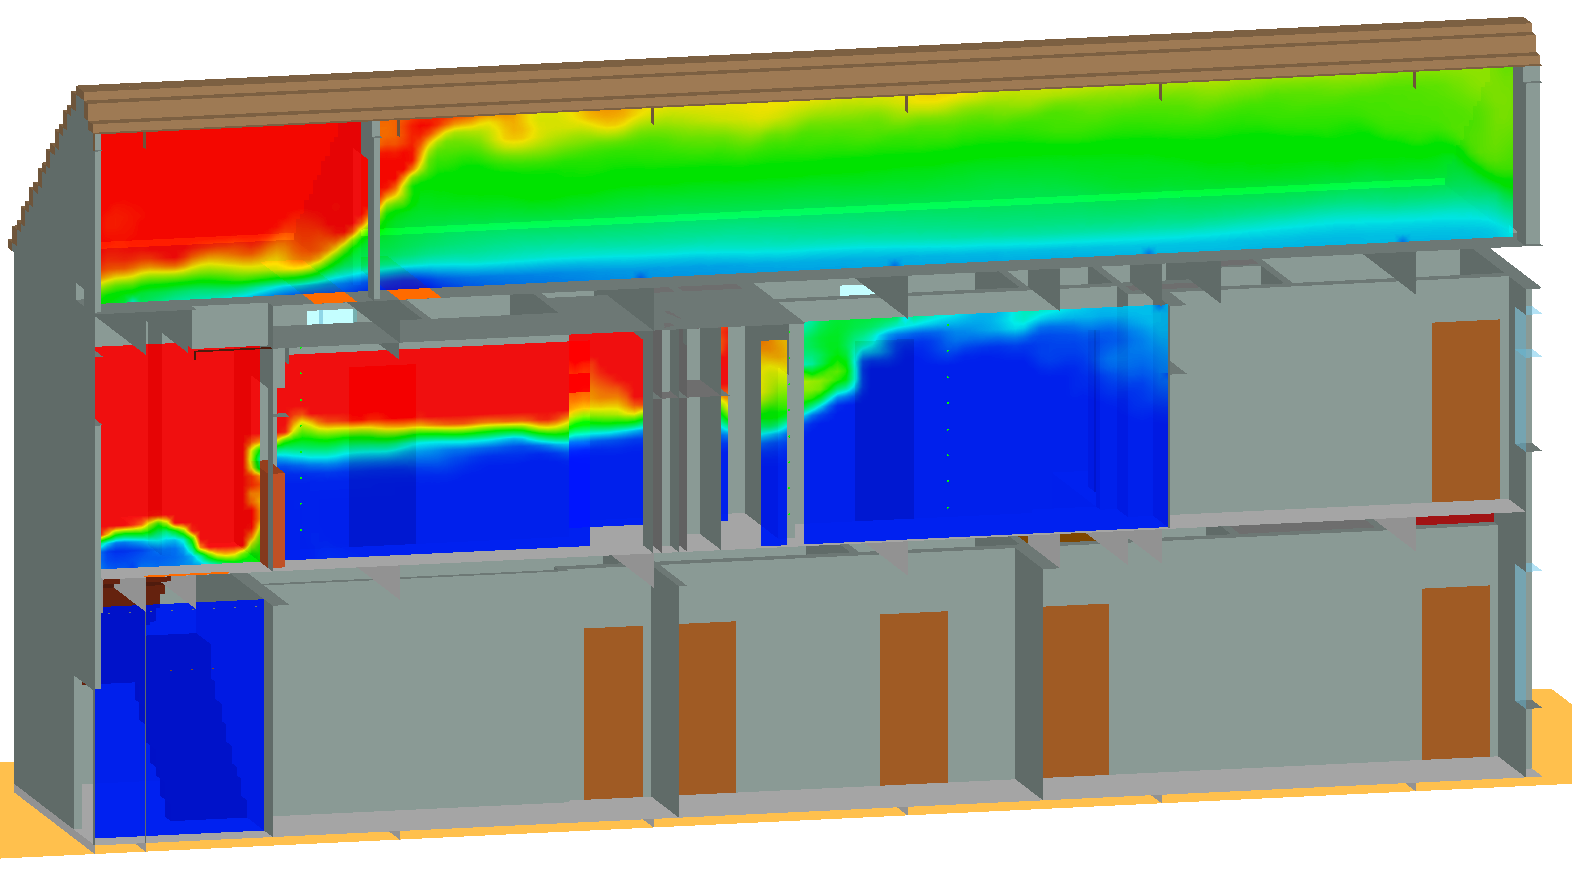
\includegraphics[width=.675\textwidth]{../Figures/west_50th_baseline_175}
%\documentclass{standalone}
%\usepackage{pgfplots}
%\begin{document}
%\pgfplotsset{
%	colormap={blackwhite}{[5pt]
%		rgb255(0pt)=(0,0,255); 
%		rgb255(100pt)=(0,255,255); 
%		rgb255(200pt)=(0,255,0); 
%		rgb255(300pt)=(255,255,0); 
%		rgb255(400pt)=(255,0,0)
%	},
%}
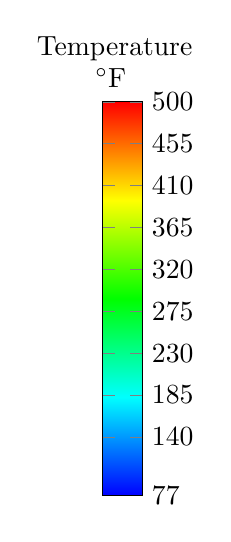
\begin{tikzpicture}
\node at (0.45,0.67) {Temperature};
\node at (0.4,0.3) {$^\circ$F};
\begin{axis}[
    hide axis,
    scale only axis,
    height=0pt,
    width=0pt,
    colorbar,
    point meta min=77,
    point meta max=500,
    colorbar style={
        height=5cm,
        ytick={77,140,185,...,500}
    }]
    \addplot [draw=none] coordinates {(0,0)};
\end{axis}
\end{tikzpicture}
%\end{document} 
%\documentclass{standalone}
%\usepackage{pgfplots}
%\begin{document}
%\pgfplotsset{
%	colormap={blackwhite}{[5pt]
%		rgb255(0pt)=(0,0,255); 
%		rgb255(100pt)=(0,255,255); 
%		rgb255(200pt)=(0,255,0); 
%		rgb255(300pt)=(255,255,0); 
%		rgb255(400pt)=(255,0,0)
%	},
%}
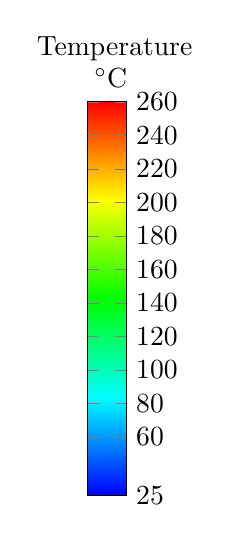
\begin{tikzpicture}
\node at (0.65,0.67) {Temperature};
\node at (0.6,0.3) {$^\circ$C};
\begin{axis}[
    hide axis,
    scale only axis,
    height=0pt,
    width=0pt,
    colorbar,
    point meta min=25,
    point meta max=260,
    colorbar style={
        height=5cm,
        ytick={25,60,80,...,260}
    }]
    \addplot [draw=none] coordinates {(0,0)};
\end{axis}
\end{tikzpicture}
%\end{document}

\caption{Temperature from baseline simulation, 15 seconds after interior door fails.}
\label{fig:temp_175s}
\end{figure}

From Fig.~(\ref{fig:temp_175s}), 15 seconds after the door failed, high temperature gases have descended to approximately 1 m (3.28 ft) off the ground through the interior hallway and have spilled into the kitchen (recall layout from Fig.~(\ref{fig:simp_geom})).


\chapter{Discussion}
The discussion will be broken up into two parts. The first part will address the results of the computational modeling as they relate to the interior hallways conditions. The second part will examine the the model results and observed outcomes of fire as they relate to tactics discussed in recent experimental research.  
\section{Conditions in Hallway}

\section{Tactical Considerations}

\chapter{Summary}

\chapter{Acknowledgements}

\bibliography{../../../Bibliography/FDS_refs,../../../Bibliography/FDS_general,chicago}

\appendix

\chapter{Dimensioned Drawings}

\begin{figure}[h!]
\centering
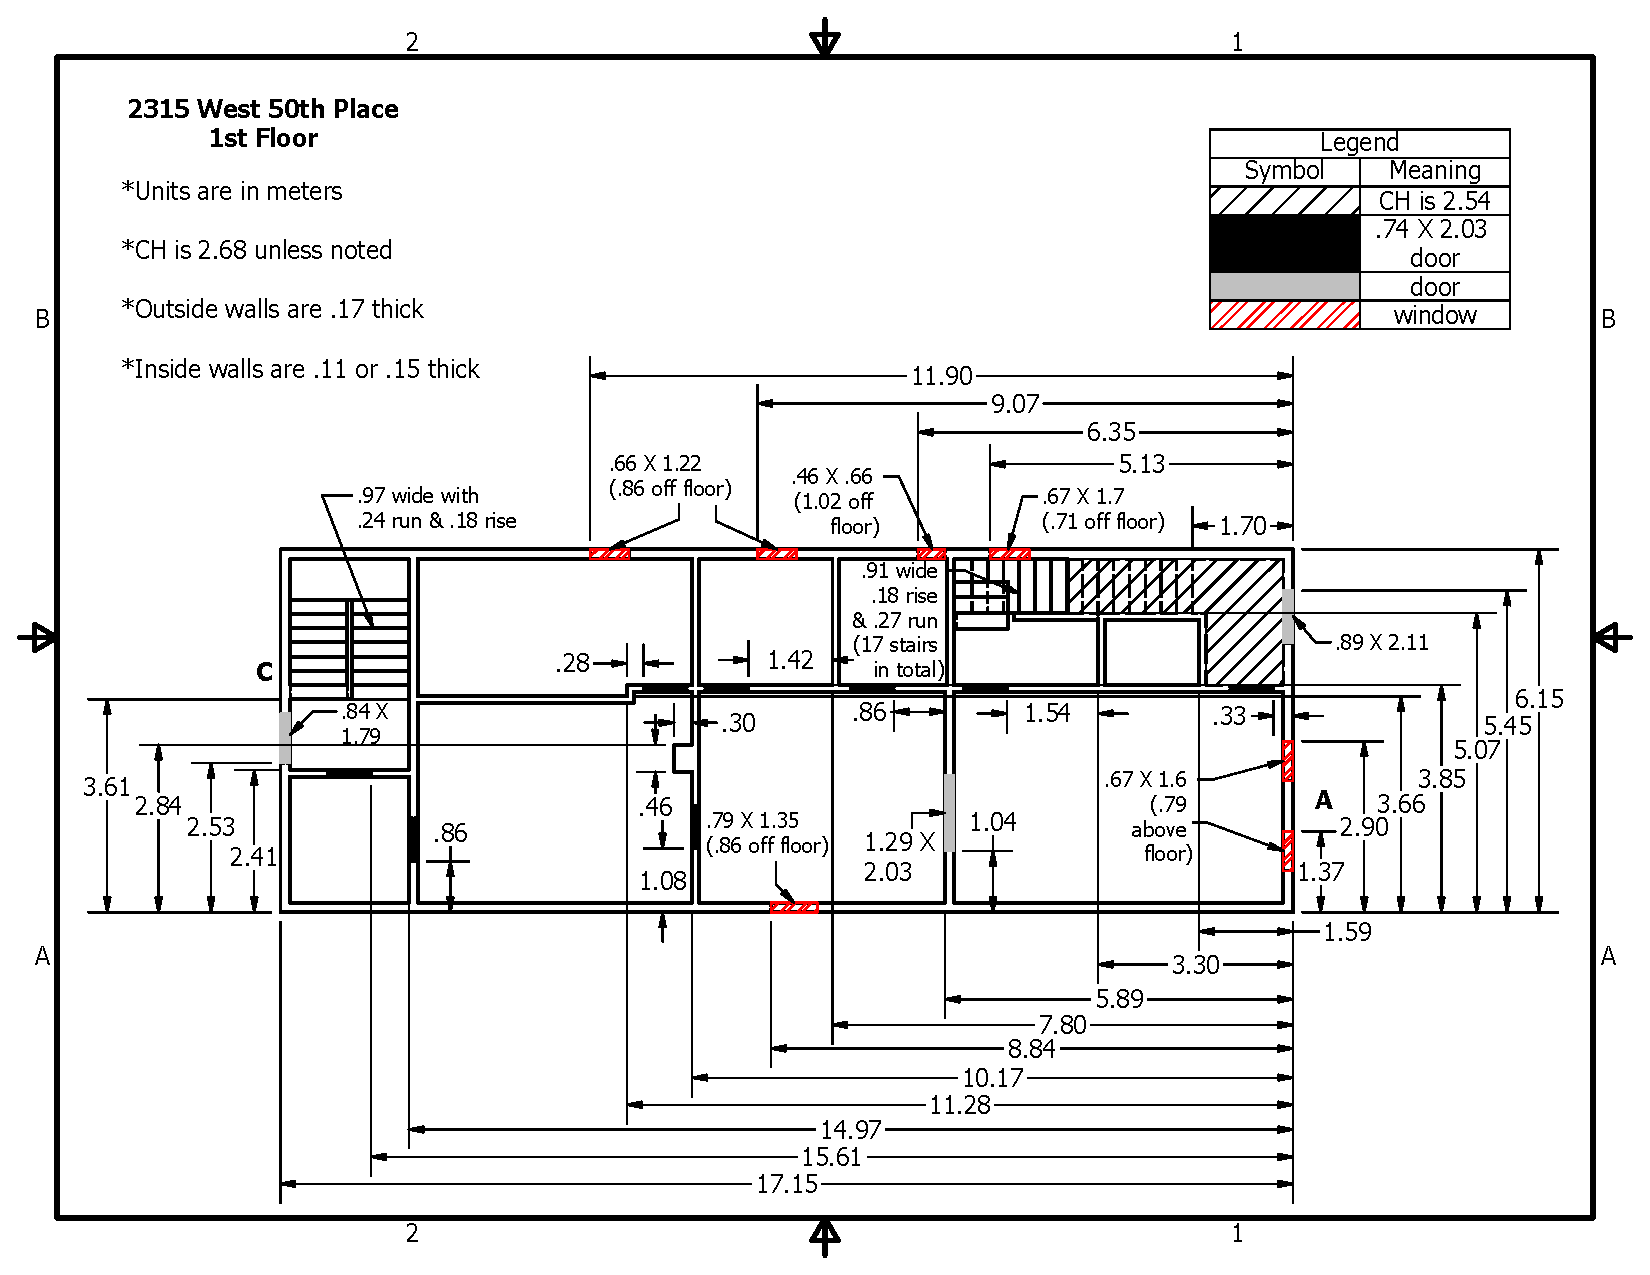
\includegraphics[width=.80\textwidth]{../Figures/50th_Place_1st_Floor}
\caption {Dimensioned drawing of 1$^{st}$ floor}
\label{fig:first_floor}
\end{figure}

\begin{figure}[h!]
\centering
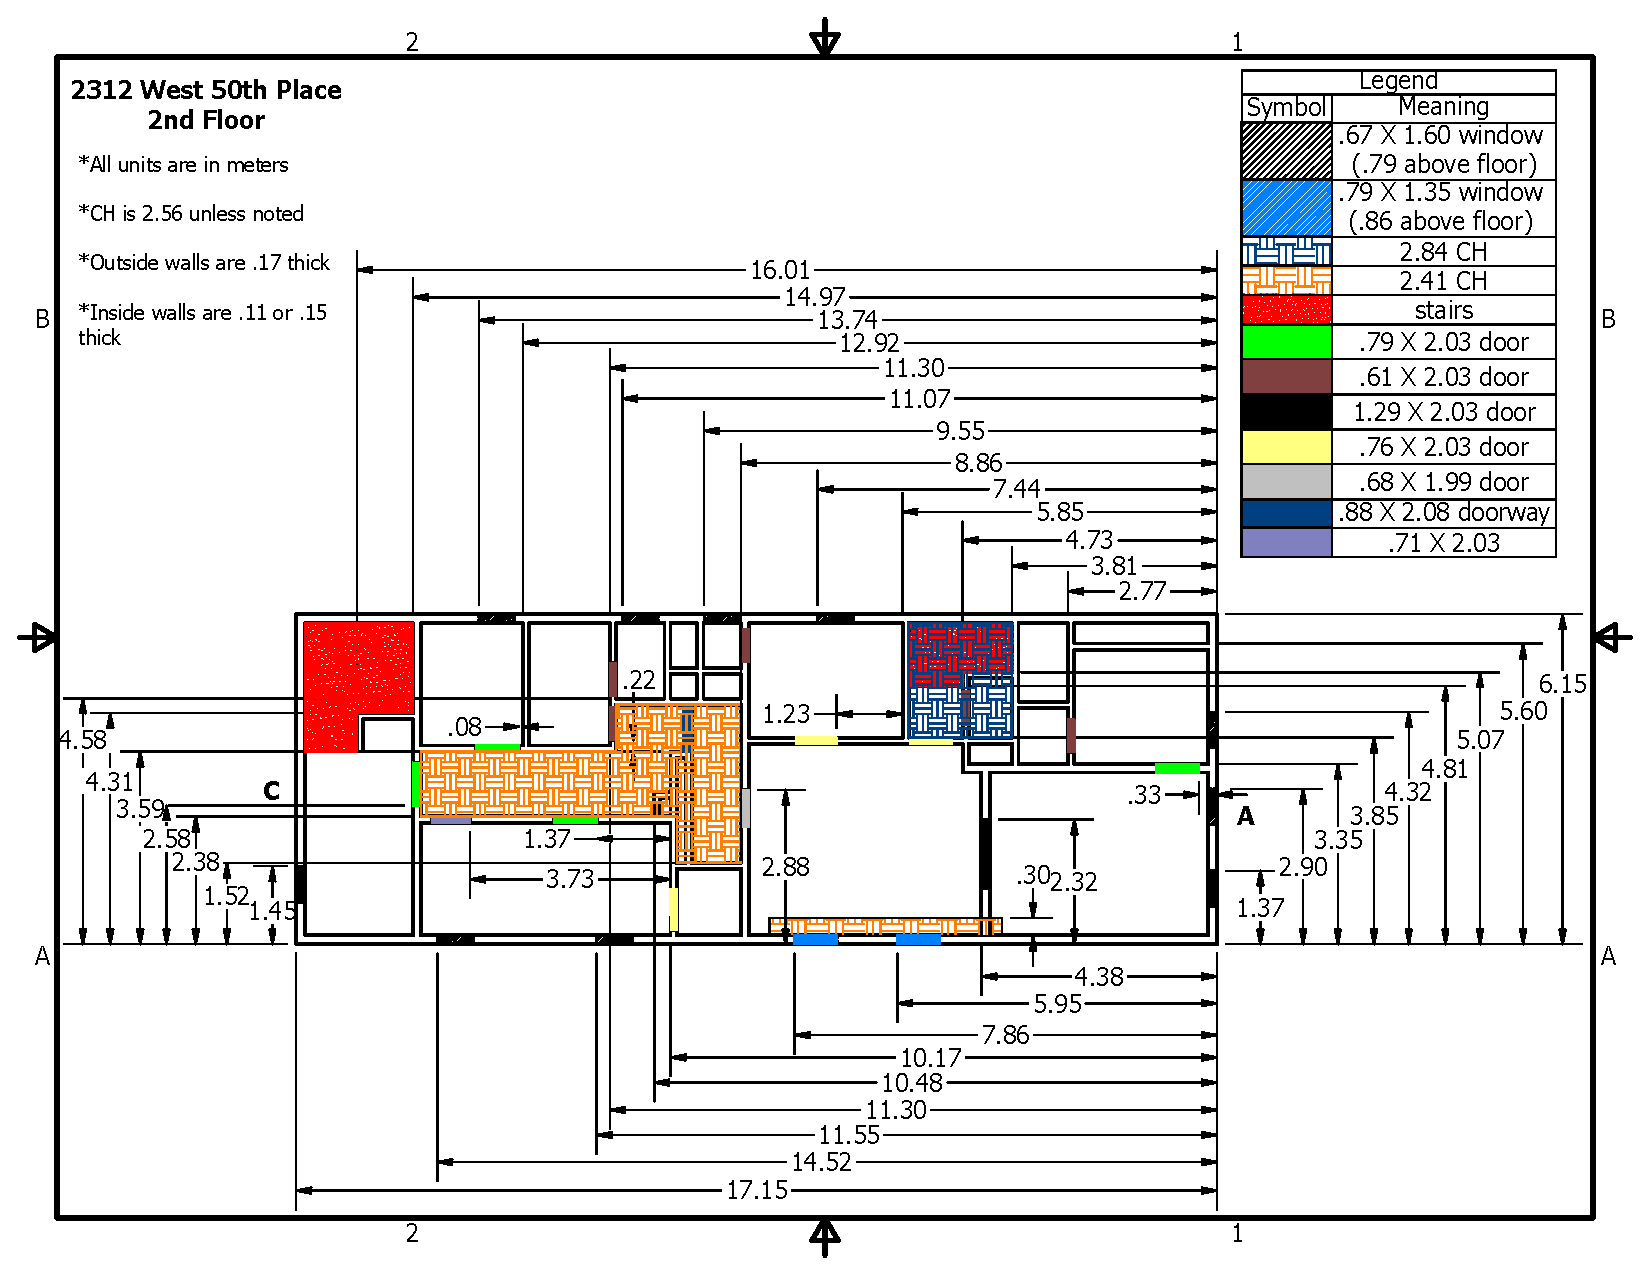
\includegraphics[width=.80\textwidth]{../Figures/50th_Place_2nd_Floor}
\caption {Dimensioned drawing of 2$^{nd}$ floor}
\label{fig:second_floor}
\end{figure}


\end{document}
